\documentclass[a4paper,oneside,12pt]{report}
\usepackage{styles/fbe_tez}
\usepackage[utf8x]{inputenc} % To use Unicode (e.g. Turkish) characters
\usepackage{amsmath, amsthm} % Some extra symbols
\usepackage[bottom]{footmisc}
\usepackage{cite}
\usepackage{graphicx}
\usepackage{longtable}
\usepackage{float}
\usepackage{multirow}
\usepackage{algorithm}
\usepackage{algorithmic}
\usepackage{array}
\usepackage{amssymb,bm,cite,graphicx, fixmath, texdraw}
\usepackage{epsfig}
\usepackage{epstopdf}
\usepackage{amsmath}
\usepackage{notoccite}
\usepackage{subcaption}
\usepackage{tabu}
\usepackage{minted}
\usepackage{xcolor}

\usemintedstyle{xcode}
\definecolor{bg}{rgb}{0.95,0.95,0.95}

\interdisplaylinepenalty=2500
\hyphenation{lists} \makeatletter

\newcommand{\field}[1]{\mathbb{#1} }
\newcommand{\beq}{\begin{equation} \setlength\abovedisplayskip{5pt} 
\setlength\belowdisplayskip{5pt}}
\newcommand{\eeq}{\end{equation}}
\newcommand{\bea}{\begin{eqnarray}}
\newcommand{\eea}{\end{eqnarray}}
\newcommand{\defn}{\stackrel{\triangle}{=}}
\newcommand{\nn}{\nonumber}
\newcommand{\nnl}{\nonumber \\}
\renewcommand{\theequation}{\arabic{equation}}
\renewcommand{\labelenumi}{(\roman{enumi})}

\DeclareMathOperator*{\argmin}{arg\,min}
\DeclareMathOperator*{\argmax}{arg\,max}

\def\ifundefined{\@ifundefined}
\def\bfat{\left[ \begin{array}}
\def\emat{\end{array} \right]}
\def\bfatt{\left\{ \begin{array}}
\def\ematt{\end{array} \right.}
\def\bset{\left\{ \begin{array}}
\def\eset{\end{array} \right\}}
\def\bpar{\left( \begin{array}}
\def\epar{\end{array} \right)}

\graphicspath{{figures/}} % Graphics will be here

\newtheorem{thm}{Theorem}[chapter]
\newtheorem{prop}[thm]{Proposition}
\newtheorem{lem}[thm]{Lemma}
\newtheorem{cor}[thm]{Corollary}

\numberwithin{equation}{chapter}

% BEGIN OF DOCS
\begin{document}
\pagenumbering{roman}


% CONTENTS AND LIST OF FIG AND TABLE PAGES
\tableofcontents

\pagenumbering{arabic}

\newcommand{\vecthreeBF}[1]{\vec{\textbf{#1}}}
\newcommand{\vecthree}[1]{\vec{#1}}

\newcommand{\parDeriv}[2]{\frac{\partial #1}{\partial #2}}
\newcommand{\parDerivS}[2]{\frac{\partial^2 #1}{\partial #2^2}}
\newcommand{\derivS}[2]{\frac{d^2 #1}{d#2^2}}

\newcommand{\dotProdBF}[2]{\vecthreeBF{#1} \cdot \vecthreeBF{#2}}
\newcommand{\dotProd}[2]{\vecthree{#1} \cdot \vecthree{#2}}

\newcommand{\crossProdBF}[2]{\vecthreeBF{#1} \times \vecthreeBF{#2}}
\newcommand{\crossProd}[2]{\vecthree{#1} \times \vecthree{#2}}


\newcommand{\fromeq}[1]{\textit{equation \ref{eq:#1}}}
\newcommand{\fromeqs}[2]{\textit{equations \ref{eq:#1} and \ref{eq:#2}}}
\newcommand{\fromeqsth}[3]{\textit{equations \ref{eq:#1}, \ref{eq:#2} and \ref{eq:#3}}}

\newcommand{\fromfig}[1]{\textit{figure \ref{fig:#1}}}
\newcommand{\fromfigs}[2]{\textit{figures \ref{fig:#1} and \ref{fig:#2}}}

\newcommand{\fromsec}[1]{\textit{section \ref{sec:#1}}}
\newcommand{\fromsecs}[2]{\textit{sections \ref{sec:#1} and \ref{sec:#2}}}

\newcommand{\fromapp}[1]{\textit{Appendix \ref{appendix:#1}}}% START OF THEORY

\chapter{THEORY}

\section{Accelerating Charged Particles}

\subsection{Relation between momentum and acceleration}
In classical mechanics, Newton's second law defines force and states 
\begin{equation} \label{eq:newton_second_law}
    \vecthreeBF{F} = \frac{\partial \vecthreeBF{p}}{\partial t} = m \frac{\partial \vecthreeBF{v}}{\partial t} = m \vecthreeBF{a}
\end{equation}
In special relativity however, relativistic momentum is defined as $\vecthree{p} = \gamma m_0 \vecthree{v} $ where $\gamma$ is the Lorentz Factor;
\begin{equation*}
    \gamma = \frac{1}{\sqrt{1-v^2 / c^2}} = \frac{1}{\sqrt{1-\beta^2}}
\end{equation*}
Considering these two statements, we can find the relation between momentum and acceleration as follows
\begin{eqnarray*}
    \parDeriv{\vecthree{p}}{t} &=& m_0 \parDeriv{(\gamma \vecthree{v})}{t} = m_0 \{  \parDeriv{\gamma}{t}\vecthree{v} + \gamma \parDeriv{\vecthree{v}}{t}  \} \\
    \parDeriv{\gamma}{t} &=& \gamma^3 \dotProd{\beta}{\parDeriv{\beta}{t}} = \frac{\gamma^3}{c} \dotProd{\beta}{a} \\
    \parDeriv{\vecthree{p}}{t}  &=& m_0 \{   \frac{\gamma^3}{c} (\dotProd{\beta}{a} )\vecthree{v} + \gamma \parDeriv{\vecthree{v}}{t}  \} 
\end{eqnarray*}
\begin{equation} \label{eq:Frel}
    \vecthreeBF{F}  = \gamma m_0 \{ \vecthreeBF{a} + \gamma^2(\dotProd{\beta}{\textbf{a}})\vecthree{\beta} \}
\end{equation}
It is clear that acceleration is not necessarily parallel to the force anymore. 

To start seperating the parallel and perpendicular components relative to $\vecthree{\beta}$, we can find $\vecthreeBF{a}_{||}$ and $\vecthreeBF{F}_{||}$.
\begin{equation} \label{eq:a_F_parallels}
    \begin{aligned}
        \vecthreeBF{a}_{||} = \frac{(\dotProd{a}{\beta})}{\beta^2}\beta 
    \end{aligned}
    \qquad \qquad
    \begin{aligned}
        \vecthreeBF{F}_{||} = \frac{(\dotProd{F}{\beta})}{\beta^2}\beta 
    \end{aligned}
\end{equation}
\begin{eqnarray*}
    \dotProd{\textbf{F}}{\beta} &=& \gamma m_0 \{ \dotProd{\textbf{a}}{\beta} + \gamma^2(\dotProd{\beta}{\textbf{a}})\beta^2 \} \\
                                &=& \gamma m_0 (\dotProd{\textbf{a}}{\beta}) \{ \gamma^2\beta^2  + 1\} 
\end{eqnarray*}
Using $\gamma^2 \beta^2 + 1 = \gamma^2 $ we have,
\begin{equation*}
    \dotProd{\textbf{F}}{\beta} = m_0 \gamma^3 (\dotProd{\textbf{a}}{\beta} )
\end{equation*}
Inserting this
\begin{eqnarray}
    \vecthreeBF{F}_{||} &=& \frac{(\dotProd{\textbf{F}}{\beta})}{\beta^2} \vec{\beta} \nonumber \\
                        &=& m_0 \gamma^3 \frac{(\dotProd{\textbf{a}}{\beta} )}{\beta^2} \vec{\beta} \nonumber \\
                        &=& m_0 \gamma^3 \vecthreeBF{a}_{||} \label{eq:Frel_parallel}
\end{eqnarray}
Therefore from \fromeqs{Frel}{Frel_parallel}
\begin{eqnarray*}
    \vecthreeBF{F}  &=& m_0 \gamma^3 \vecthreeBF{a}_{||} \beta^2 + m_0 \gamma \vecthreeBF{a} \\
                    &=& m_0 \gamma^3 \vecthreeBF{a}_{||} \beta^2 + m_0 \gamma \{ \vecthreeBF{a}_{||} +  \vecthreeBF{a}_{\perp} \} \\
                    &=& m_0 \vecthreeBF{a}_{||} \gamma \{ \gamma^2\beta^2 + 1 \} + m_0 \gamma \vecthreeBF{a}_{\perp} \\
                    &=& m_0 \vecthreeBF{a}_{||} \gamma^3 + m_0 \gamma \vecthreeBF{a}_{\perp} \\
                    &=& \vecthreeBF{F}_{||} + m_0 \gamma \vecthreeBF{a}_{\perp}
\end{eqnarray*}
We finally have two seperate equations which are in similar form with \fromeq{newton_second_law}.
\begin{equation} \label{eq:Frel_para_and_perp}
    \begin{aligned}
        \vecthreeBF{F}_{||} = \gamma^3  m_0 \vecthreeBF{a}_{||}
    \end{aligned}
    \qquad \qquad
    \begin{aligned}
        \vecthreeBF{F}_{\perp} = \gamma  m_0\vecthreeBF{a}_{\perp}
    \end{aligned}
\end{equation}


\subsection{Lorentz Force} \label{sec:lorentz-force}
Force acting on a charged particle moving in electromagnetic fields is called Lorentz Force and is given by the formula
\newline
\begin{equation} \label{eq:lf}
    \frac{\partial \vecthree{p}}{\partial t} = \vecthree{F}_L=q(\vecthree{E}+ \vecthree{v} \times \vecthree{B})
\end{equation}
\newline
where the $q$ is the charge and $\vecthree{v}$ is the velocity of the particle. 

\subsection{Relativistic Lorentz Force}
Similar to non-relativistic version, relativistic Lorentz Force is given by the following 4-vector equality
\begin{equation}
    \frac{\partial p^{\mu}}{\partial \tau} = q F^{\mu \nu} u_{\nu}
\end{equation}
Where $ \partial \tau = \partial t / \gamma $,
\begin{equation}
    \begin{aligned}
        p^{\mu} = 
        \begin{bmatrix}
            W/c \\
            p_x         \\
            p_y \\
            p_z
        \end{bmatrix}    
    \end{aligned}
    \qquad\qquad
    \begin{aligned}
        F^{\mu\nu} = 
        \begin{bmatrix}
                0       & -E_x/c   & -E_y/c    & -E_z/c \\
                E_x/c   &   0      & -B_z      & B_y     \\
                E_y/c   &   B_z    &  0        & -B_x     \\
                E_z/c   &   -B_y   & B_x       & 0   
        \end{bmatrix} 
    \end{aligned}
    \qquad\qquad
    \begin{aligned}
        u_{\nu} = \gamma
        \begin{bmatrix}
                 c \\
                -v_x \\
                -v_y \\
                -v_z \\
        \end{bmatrix} 
    \end{aligned}
\end{equation}
Where $W$ is the energy of the particle and $\gamma$ is the lorentz factor mentioned in the previous section.
\newline

For $ \mu = 0 $, we have the time component of the equation;
\begin{eqnarray}
    \frac{\gamma}{c}\frac{\partial W}{\partial t} &=& \frac{q \gamma \vecthree{E}\cdot \vecthree{v}}{c} = \frac{q \gamma}{c}  \frac{\vecthree{E}  \cdot \partial \vecthree{r}}{\partial t} \\
    \frac{\partial W}{\partial t} &=& q \frac{\vecthree{E}\cdot \partial \vecthree{r}} {\partial t}
\end{eqnarray}
This is the definition of work done by an electric field. For $ \mu = 1,2,3 $, we have the spacial components;
\begin{equation*}
    \frac{\partial \vecthree{p}}{\partial \tau} = \gamma \frac{\partial \vecthree{p}}{\partial t} = q \gamma (\vecthree{E} + \vecthree{v} \times \vecthree{B})
\end{equation*}
Which simplifies to non-relativistic Lorentz Force in \fromeq{lf}.


\subsection{Acceleration caused by lorentz force}
Due to the nature of the cross product, lorentz force caused by a magnetic field is always perpendicular to the velocity of the particle. 
Therefore the acceleration of the magnetic field is straightforward
\begin{equation*}
    \vecthreeBF{F}_B = \vecthreeBF{F}_{\perp} = \gamma  m_0\vecthreeBF{a}_{\perp} = \gamma  m_0\vecthreeBF{a}_{B}
\end{equation*}
The same thing cannot be said about electric field however. 
It can create force in any direction with respect to velocity. Therefore, we have the following equality;
\begin{equation} \label{eq:para_and_perp_acc_of_lorentz_force}
    \begin{aligned}
        \vecthreeBF{a}_{||} = \frac{q }{\gamma^3 m_0} \vecthreeBF{E}_{||}
    \end{aligned}
    \qquad \qquad
    \begin{aligned}
        \vecthreeBF{a}_{\perp} = \frac{q}{\gamma m_0} \{ \vecthreeBF{E}_{\perp} + \crossProdBF{v}{B}   \}
    \end{aligned}    
\end{equation}
Acceleration due to electric field can be simplified as;
\begin{eqnarray*}
    \vecthreeBF{a}_{\{B=0\}} = \vecthreeBF{a}_{E}   &=&  \vecthreeBF{a}_{||} + \vecthreeBF{a}_{\perp \{B=0\}} \\
                                &=& \frac{q}{m_0 \gamma} \{ \frac{\vecthreeBF{E}_{||}}{\gamma^2} + \vecthreeBF{E}_{\perp} \} \\
                                &=& \frac{q}{m_0 \gamma} \{ \{1 - \beta^2\}\vecthreeBF{E}_{||} + \vecthreeBF{E}_{\perp} \} \\
                                &=& \frac{q}{m_0 \gamma} \{ \vecthreeBF{E}_{||} + \vecthreeBF{E}_{\perp}-\beta^2\vecthreeBF{E}_{||} \} \\
                                &=& \frac{q}{m_0 \gamma} \{ \vecthreeBF{E} - \beta^2\vecthreeBF{E}_{||} \} \\
\end{eqnarray*}
Using the fact that $\vecthreeBF{E}_{||} = \vec{\beta}(\dotProd{\textbf{E}}{\beta})/\beta^2 $, we finally have
\begin{equation} \label{eq:acc_of_E_and_B}
    \begin{aligned}
        \vecthreeBF{a}_{E} = \frac{q}{ \gamma m_0} \{ \vecthreeBF{E} - \vecthreeBF{v}\frac{(\dotProdBF{E}{v})}{c^2} \}
    \end{aligned}
    \qquad \qquad
    \begin{aligned}
        \vecthreeBF{a}_{B} = \frac{q}{\gamma m_0} ( \crossProdBF{v}{B} )
    \end{aligned}
\end{equation}

\newpage



\section{Particle Accelerators}

Particle accelerators are sophisticated scientific instruments designed to accelerate charged particles, such as electrons, protons, or ions, to high speeds and energies. 
These accelerators play a crucial role in advancing our understanding of the fundamental properties of matter and the universe. 
They are widely used in various fields of research, including particle physics, nuclear physics, materials science, and medicine.

At their core, particle accelerators utilize electromagnetic fields to impart energy to particles and control their trajectories. 
These fields are generated by intricate arrangements of magnets and RF (radiofrequency) cavities within the accelerator structure. 
By precisely controlling these fields, accelerators can propel particles to speeds close to the speed of light, enabling them to acquire high energies.

Accelerators can be categorized into two main types: linear accelerators (linacs) and circular accelerators. 
Linacs accelerate particles in a straight line, while circular accelerators use magnetic fields to bend the particle trajectory into a circular path. 

The acceleration process in accelerators involves multiple stages. Initially, particles are injected into the accelerator at a relatively low energy. 
As they progress through the accelerator, they are subjected to alternating electric fields that accelerate them, while magnetic fields guide their trajectories.
Focusing elements, such as magnetic lenses or quadrupole magnets, ensure the particles remain tightly controlled.

As particles gain energy in the accelerator, they approach relativistic speeds, where relativistic effects become significant. 
Special relativity governs the increase in mass and energy of the particles as they approach the speed of light, providing insights into the behavior of matter at high energies.

Particle accelerators are essential tools for scientific research. They enable scientists to probe the fundamental constituents of matter, study particle interactions, and explore the laws of physics. 
Accelerators have been instrumental in discovering and characterizing fundamental particles, such as quarks, leptons, and the Higgs boson. 
They also facilitate the production of high-intensity beams for applications in material science, radiotherapy, and industrial processes like particle irradiation and sterilization.

% TODO : ADD CIRCULAR AND LINEAR ACCELERATOR PICTURES HERE
\begin{figure}[H]
    \centering
    
\includegraphics[scale=0.75]{./figures/to_be_added.png}
    \caption{A circular accelerator}
\end{figure}

\begin{figure}[H]
    \centering
    
\includegraphics[scale=0.75]{./figures/to_be_added.png}
    \caption{A linear accelerator}
\end{figure}

\subsection{Key Concepts}

\begin{itemize}
    \item Phase Stability
    \item Phase Lag
    \item Shunt Impedance
    
\end{itemize}

\subsection{Acceleration Cavities} \label{sec:theory_cavities}
Radiofrequency (RF) cavities, also known as accelerating cavities or resonant cavities, are key components in particle accelerators. 
These cavities generate strong electromagnetic fields at specific frequencies to accelerate charged particles through clever engineering.

RF cavities are typically hollow metallic structures made of or coated with high-conductivity materials such as copper. 
They are designed to resonate at a specific frequency, which is determined by the size and shape of the cavity. 
The cavity is often cylindrical or spherical in shape, and its inner surface is polished to minimize energy losses through resistive heating.
The RF cavity is designed to be resonant, meaning that it naturally amplifies the electric fields at its resonant frequency. 
The resonant frequency is determined by the cavity's dimensions and the speed of light in the cavity material.

To achieve efficient energy transfer to the particles, the RF cavity is driven by an external RF power source operating at the resonant frequency. 
The power source supplies radiofrequency energy to the cavity, which causes the electric fields inside the cavity to oscillate at the desired frequency. 
These oscillating fields then transfer energy to the passing particles, increasing their kinetic energy by pushing and pulling on the charged particles as they pass through the cavity. 

In addition to accelerating the particles, RF cavities are often designed to provide focusing forces. 
By carefully shaping the cavity and adjusting the electromagnetic fields, the particles can experience focusing effects as they pass through the cavity. 
This helps to maintain a tight and controlled beam. To ensure efficient acceleration, it is essential to maintain phase stability. 
This means that the particles should experience the strongest electric fields at the correct time during their passage through the cavity. 
Precise timing and synchronization of the RF power source with the particle beam are crucial to achieve phase stability and maximize energy transfer.
% TODO : ADD RF CAVITY PICTURE HERE
\begin{figure}[H]
    \centering
    
\includegraphics[scale=0.75]{./figures/to_be_added.png}
    \caption{A rf cavity used in KAHVELab}
\end{figure}

\subsection{Steerer Magnets}
Steerer magnets, also known as dipole magnets or bending magnets, are fundamental components used in particle accelerators to control the trajectory of charged particles. 
They utilize the Ampere's Law to exert a magnetic field that interacts with the charged particles in the accelerator. 

According to the Lorentz Force Law ( $\textit{Section \ref{sec:lorentz-force}}$ ), when a charged particle moves through a magnetic field, it experiences a force perpendicular to both its velocity 
vector and the magnetic field direction. This force causes the particle's trajectory to curve, resulting in a bending effect.

% TODO : ADD STEERER MAGNET PICTURE HERE
\begin{figure}[H]
    \centering
    
\includegraphics[scale=0.75]{./figures/to_be_added.png}
    \caption{A steerer magnet used in KAHVELab}
\end{figure}

\subsection{Rhodotron Accelerator} \label{sec:theory_rhodo}

Rhodotron Accelerator is a type of particle accelerator that was proposed by \textit{Jacques POTTIER} in his publication \textit{A new type of rf electron accelerator:The Rhodotron} in 1989 \cite{rhodo_pottier}. 
First prototype was built at CEA Saclay later in 1992 \cite{rhodo_prototype}. Its named after the greek word for rose, \textit{rhodos}, due to the shape of the design \cite{rhodos}.

The design of a rhodotron mainly consists of a coaxial cylindrical RF cavity and steerer magnets surrounding it. RF cavity is fed by an external RF source, accelerating the electrons entering from an attached electron gun.

\subsubsection{Cavity of a Rhodotron} \label{sec:cavity_of_a_rhodotron}

Coaxial design of the cavity concentrates the electric field, while the magnetic field diminishes in the middle of the cylinders. 
Therefore the electrons are injected and accelerated in the plane of zero magnetic field where the electric field is strongest.
% TODO : ADD SUPERFISH AND CST SIMULATIONS OF A SIMPLE RHODOTRON CAVITY

\begin{figure}[H]
    \centering
    
\includegraphics[scale=0.75]{./figures/to_be_added.png}
    \caption{SUPERFISH simulation of a coaxial cavity}
\end{figure}

\begin{figure}[H]
    \centering
    
\includegraphics[scale=0.75]{./figures/to_be_added.png}
    \caption{CST simulation of a coaxial cavity}
\end{figure}

With the expectation that the electrons will accelerate to speeds $>=0.9 c$ after the first pass, a rhodotron cavity is designed so that the length of the path between successive passes is an integer multiple of $\lambda$, wavelength of the RF field ($l=p\lambda \label{eq:lpl}$).
This constraint helps with  phase stability and synchronization of the beam.

In the table below, optimized characteristics of a rhodotron cavity can be observed. 
\begin{figure}[H]
    \centering
    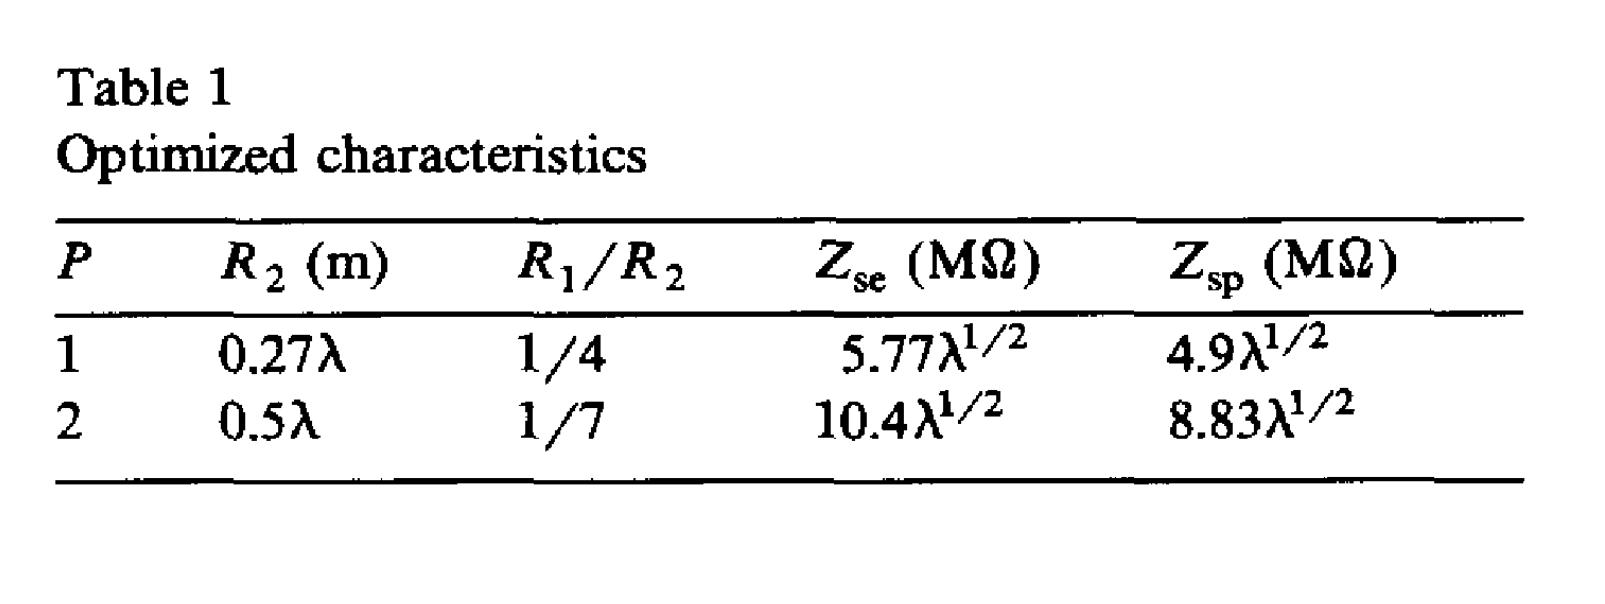
\includegraphics[width=.9\textwidth]{./figures/pottier_table1.png}
    \caption{Optimized characteristics of a rhodotron cavity \cite{rhodo_pottier}}
    \label{fig:pottier_table1}
\end{figure}

Here, $p$ is the integer multiplier in the equation ($l=p\lambda$) mentioned above, $R_1$ is the radius of the inner cylinder, $R_2$ is the radius of the outer cylinder, 
$Z_{se}$ is effective shunt empedance, $Z_{sp}$ is practical shunt empedance which was taken to be $0.85 Z_{se}$.

Energy gain after each pass can be calculated by the following formula \cite{rhodo_pottier}
\begin{equation}
    \label{eq:W_gain_each_pass_pottier}
    W_1 = Z_{sp}^{1/2} P^{1/2} cos \phi  
\end{equation}

Where $P$ is the dissipated power, $\phi$ is the phase lag, taken as $15^\circ$ \cite{rhodo_pottier}. 

Considering $Z_{sp} \propto \lambda^{1/2}$, \,\,\, $W_1 \propto \lambda^{1/4}$, \,\,\,   $V \propto \lambda^3$, where $V$ is the volume of the cavity, implementing the $p=1$ design in \fromfig{pottier_table1} is much more space efficient.
\begin{figure}[H]
    \centering
    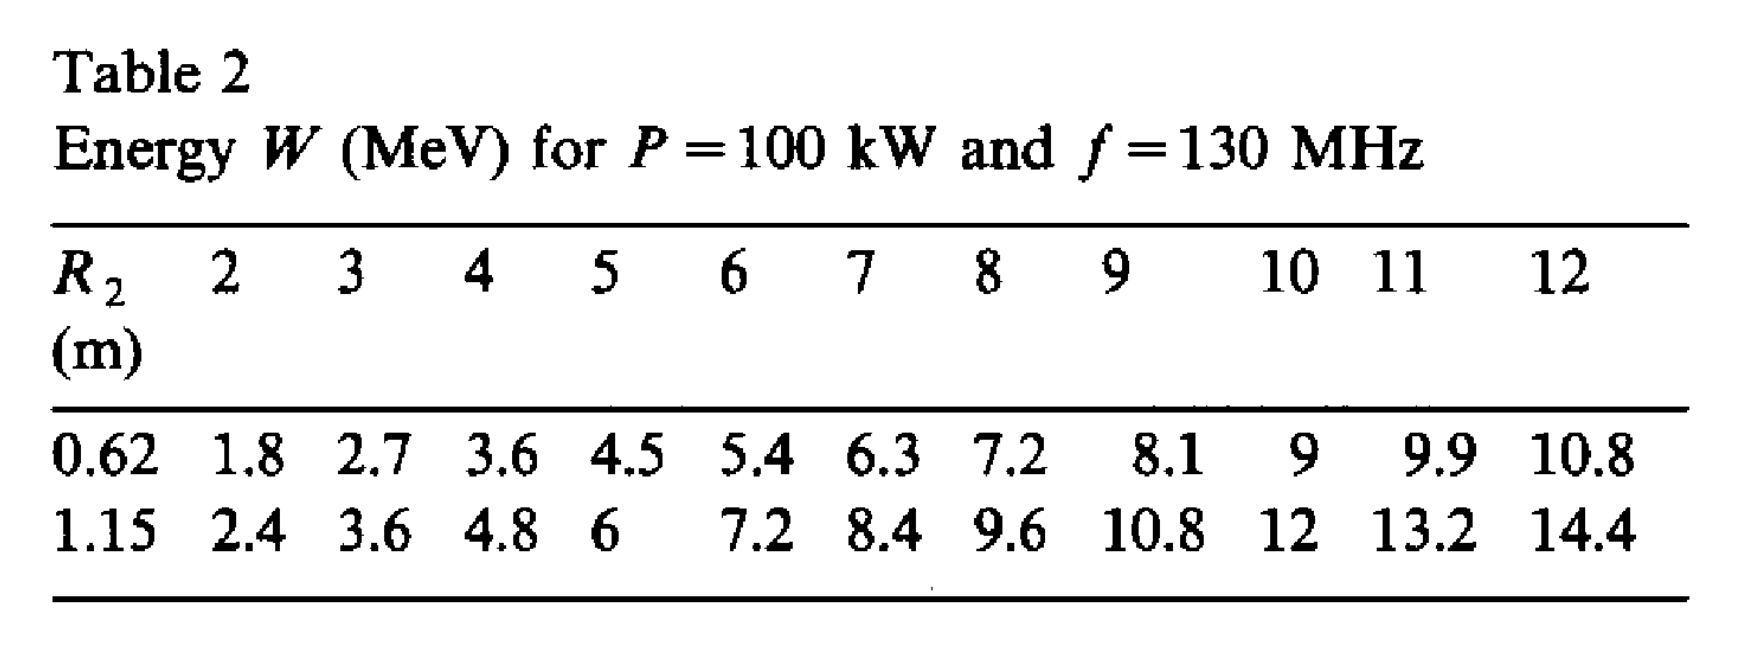
\includegraphics[width=.9\textwidth]{./figures/pottier_table2.png}
    \caption{Energy of a synchronous electron after each pass for both $p=1$ and $p=2$ \cite{rhodo_pottier}}
    \label{fig:pottier_table2}
\end{figure}

Total energy gain after n passes $W$ can then be found by \fromeq{W_gain_each_pass_pottier}, taking $\phi = 15^\circ$, $p=1$, i.e $R_2 = 0.27 \lambda$.
\begin{equation}
    \label{eq:W_total_gain_pottier}
    W \approx 2.14 \lambda^{1/4} P^{1/2} n \quad keV
\end{equation}

\subsubsection{Acceleration cycle of Rhodotron}

Electrons undergo four different stages during a single pass. 
They are accelerated between the cylinderical plates and are shielded from the changing RF field while inside the inner cylinder and outside the cavity. 

\begin{description}
    \item[First acceleration] Electrons in the rhodotron cavity are accelerated by the electric field created between two coaxial cylinders, towards the inner cylinder when they are ejected into the cavity.
    \item[Inner shielding] While inside the inner cylinder, the cylinder acts as a faraday cage and shields the electrons inside while the electric field is being reversed.
    \item[Second acceleration] Once the electrons leave the inner cylinder, they accelerate towards the outer cylinder by the reversed electric field until they leave the cavity.
    \item[Magnets] After leaving the cavity, an electromagnet placed in their path steers the electrons back into the cavity in which time the electric field changes the direction again.
\end{description}

This cycle can be repeated as long as real world constraints such as; placements and dimentions of the electromagnets, power requirements due to increasing magnetic field in order for sharper turns, can be overcomed.
After desired amount of pass has been completed, the electrons exit the accelerator.

This process is explained further in the following figures where $T$ is the period of the electric field.
% TODO : ADD ACCELERATION PROCESS OF RHODOTRON FIGURES HERE
\begin{figure}[H]
    \centering
    
\includegraphics[scale=0.75]{./figures/to_be_added.png}
    \caption{$[0, \frac{T}{4}]$ time frame of a rhodotron}
\end{figure}

\begin{figure}[H]
    \centering
    
\includegraphics[scale=0.75]{./figures/to_be_added.png}
    \caption{$[\frac{T}{4}, \frac{T}{2}]$ time frame of a rhodotron}
\end{figure}

\begin{figure}[H]
    \centering
    
\includegraphics[scale=0.75]{./figures/to_be_added.png}
    \caption{$[\frac{T}{2}, \frac{3T}{4}]$ time frame of a rhodotron}
\end{figure}

\begin{figure}[H]
    \centering
    
\includegraphics[scale=0.75]{./figures/to_be_added.png}
    \caption{$[\frac{3T}{4}, T]$ time frame of a rhodotron}
\end{figure}




\newpage



\section{Numerical Integration Methods}

\subsection{Leapfrog} \label{sec:leapfrog}
The Leapfrog method is a numerical method commonly used to solve ordinary differential equations (ODEs) that involve second-order time derivatives. Such an ODE is shown below:

\begin{equation}
    \ddot{x} = \derivS{x}{t} = f(x) \label{eq:second-order-ODE}
\end{equation}
\newline
The Leapfrog method is a variant of the finite difference method, and it approximates the solution of an ODE by discretizing both time and space. The method gets its name from the way it calculates the values of the solution at each time step, which resembles a "leapfrogging" motion. 
It is a simple and efficient algorithm that is often used in simulations of physical systems, such as celestial mechanics or molecular dynamics.
The idea is straight forward; in the time interval $\Delta t$, 
\begin{eqnarray}
    a(t_0) &=& f(x_0) \nonumber \\
    x(t_0 + \Delta t) &=& x(t_0) + v(t_0)\Delta t + a(t_0)\frac{\Delta t^2}{2} \label{eq:leapfrog_sync_x}\\
    v(t_0 + \Delta t) &=& v(t_0) + \{ a(t_0) + a(t_0 + \Delta t)\}\frac{\Delta t}{2}  \label{eq:leapfrog_sync_v}
\end{eqnarray}

For more stability, this version can be rearranged to what is called 'kick-drift-kick' form,
\begin{eqnarray} \label{eq:leapfrog}
    v(t_0 + \Delta t/2) &=& v(t_0) +  a(t_0)\frac{\Delta t}{2} \nonumber \\
    x(t_0 + \Delta t) &=& x(t_0) + v(t_0 + \Delta t/2)\Delta t \\
    v(t_0 + \Delta t) &=& v(t_0 + \Delta t/2) + a(t_0 + \Delta t)\frac{\Delta t}{2}  \nonumber
\end{eqnarray}

This version provides more time resolution to our calculation; however, it increases the number of calculations needed by about $50\%$.

\subsection{Runge Kutta}

The Runge-Kutta methods, named after the German mathematicians Carl Runge and Martin Wilhelm Kutta, family of numerical methods
used to solve ordinary differential equations (ODEs) that are in the following form

\begin{equation} \label{eq:first-order-ODE}
    \parDeriv{y}{x} = f(x, y)
\end{equation}


The basic idea behind the Runge-Kutta method is to approximate the solution of an ODE by taking small steps and using a weighted average 
of function evaluations at different points within each step.

\begin{equation} \label{eq:general-rk}
    \begin{aligned}
        y_{n+1} = y_n + \delta x \sum_{i=1}^{m} b_i k_i
    \end{aligned}
    \qquad
    \begin{aligned}
        x_{n+1} = x_n + \delta x 
    \end{aligned}
\end{equation}
where 
\begin{eqnarray} \label{eq:general-rk-coef}
    k_i = f(x_n + c_i \delta x, y_n + \delta x \sum_{j = 1}^{i - 1}a_{ij}k_j)
\end{eqnarray}

These \fromeqs{general-rk}{general-rk-coef} define the family of methods. To specify a perticular method, order $m$, coefficients $a_{ij}$, $b_i$ and $c_i$ should be provided.
The coefficients of any Runge-Kutta method can be visualized by a tableau called $\textit{Butcher Tableau}$.

\begin{figure}[h!]
    \[ 
    \begin{array} 
        {c|cccc}
        0\\
        c_1 & a_{21} \\
        c_2 & a_{31} & a_{32}\\
        \vdots& & \cdots& \\
        c_m & a_{m1} & a_{m2} & \cdots & a_{m,m-1}\\
        \hline
        & b_1 & b_2 &\cdots & b_m
    \end{array}
    \]
    \caption{Butcher Tableau}
    \label{fig:Butcher}
\end{figure}

The simplest Runge-Kutta method is the \textit{Euler's method}. Its \textit{Butcher tableau} is as follows.
\[ 
    \begin{array} 
        {c|cccc}
        0\\
        \hline
        & 1
    \end{array}
\]


The most commonly used version of the Runge-Kutta method is the fourth-order Runge-Kutta method, also known as RK4. 
The RK4 method involves four function evaluations per step and has an error term that is proportional to the step size raised to the fifth power.
Two of the most used \textit{Butcher tableaus} for \textit{RK4} given below.


\begin{figure}[h!]
    \centering
    \begin{subfigure}{.5\textwidth}
        \[ 
        \begin{array} 
            {c|cccc}
            0\\
            1/2 & 1/2 \\
            1/2 & 0 & 1/2 \\
            1   & 0 & 0 & 1\\
            \hline
            & 1/6 & 1/3 & 1/3 & 1/6
        \end{array}
        \]  
    \end{subfigure}%
    \begin{subfigure}{.5\textwidth}
        \[ 
        \begin{array} 
            {c|cccc}
            0\\
            1/3 & 1/3 \\
            2/3 & -1/3 & 1 \\
            1   & 1 & -1 & 1\\
            \hline
            & 1/8 & 3/8 & 3/8 & 1/8
        \end{array}
        \]  
    \end{subfigure}
    \caption{Butcher Tableau for RK4}
    \label{fig:Butcher-RK4}
\end{figure}

The second tableau in \fromfig{Butcher-RK4} is called the \textit{"3/8 rule"}. Its main advantage is that its error coefficients are smaller than the other. But it costs more floating point operations per step. 
Resulting in slower calculations. 



\newpage



\section{Simulation}


A simulation software is a computer program or tool that enables the creation and execution of 
simulations to model and analyze real-world systems or processes. 
It allows users to replicate the behavior, interactions, and outcomes of the system or process under study, 
providing insights and predictions that can be valuable for decision-making, optimization, or understanding complex phenomena.

Simulation software provides a virtual environment where users can define the parameters,
variables, and rules of the system being simulated. The software then uses mathematical and physical models, 
algorithms, and computational techniques to simulate the behavior of the system over time.

\subsection{Basic Consepts in Programming}

\subsubsection{Clock Cycle}

In programming, a clock cycle refers to a fundamental unit of time measurement used in computer systems. 
It represents the basic rhythm or timing mechanism of a computer's central processing unit (CPU) and is typically measured in terms of the CPU's clock speed, expressed in hertz (Hz).

A clock cycle represents one complete pulse or oscillation of the CPU's clock signal. 
It serves as a synchronization mechanism, coordinating the execution of instructions and the timing of various operations within the CPU.
Each clock cycle is associated with a specific duration, which is determined by the clock speed of the CPU.

The concept of clock cycles is often used when considering the performance and efficiency of algorithms and code. 
Since the execution time of instructions is influenced by the number of clock cycles required, minimizing the number of clock cycles needed for a program or algorithm can lead to faster and more efficient code execution.
Table below shows the amount of clock cycles required for some mathematical calculations in various processors.

\begin{figure}[h!]
    \centering
    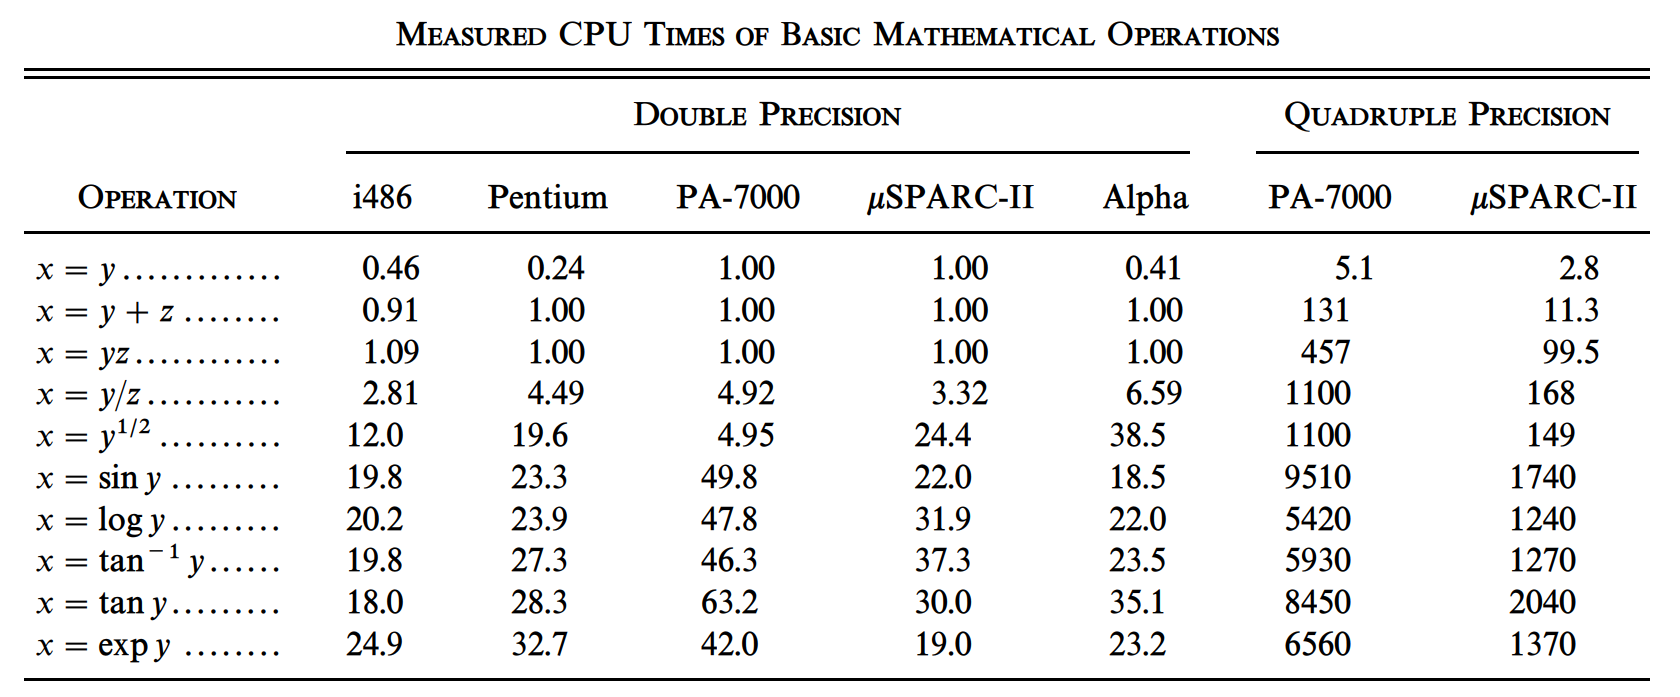
\includegraphics[width=.9\textwidth]{./figures/cpu_instruction_speed.png}
    \caption{Amount of clock cycle for mathematical operations in various processors. \cite{cpu_instruction_speed}}
\end{figure}

Note that \textit{division} is by far the most time consuming basic mathematical operation between addition, subtraction and multiplication.

\subsubsection{Concurrency}

Concurrency in programming refers to the ability of a program to execute multiple tasks or processes simultaneously. It allows different parts of a program to make progress independently, potentially improving performance, responsiveness, and resource utilization.

Concurrency in single core can be achieved by implementing clever scheduling of list of operations called \textit{threads}. This results in non-blocking execution of multiple threads, but only one thread would be executed at any given time. 
True concurrency on the other hand, can only be achieved by using multiple cores. Each core would be able to execute one thread at any time.

Programs that implement concurrency using multiple cores executes more operations per clock cycle. However, this does not directly lead to an improved performance due to the heavy burden of scheduling and managing multiple threads.




\newpage

% START OF DESIGN

\chapter{DESIGN}

\section{Cavity Design} \label{sec:cavity_design}

The first and the most important design parameter for a cavity is the operating RF frequency.
After an operating RF frequency is set and the desired $R1/R2$ relation \fromfig{pottier_table1} is selected, design parameters of acceleration plane of the cavity is fully determined.

By following the cylinderical design mentioned in \fromsec{theory_rhodo}, the only main design parameter remaining is the height of the cylindrical cavity.
This parameter can be found using the constraint mentioned in \fromsec{theory_cavities}; the fact that operating RF frequency must be equal to resonant frequency of the cavity.
For simple coaxial cavity, the height should be $\lambda/2$, where $\lambda$ is the wavelength of the external RF supply \cite{rhodo_pottier}.
Simulation tools such as \textit{CST Studio}, \textit{Poisson SUPERFISH} can be used to confirm this condition.

In the following examples, $p=1$ from \fromfig{pottier_table1} was used, and \textit{it will be the focus of all further calculations.}
Using $f_{RF}=107.5$ MHz, $f_{RF}=180$;
\begin{eqnarray} \label{eq:107_180_MHZ_cavity_design_parameters}
    \begin{aligned}
        f_{107.5} = 107.5 \textrm{ MHz} \\
        \lambda_{107.5}  = \frac{c}{f_{107.5}} = 2.789 m \\
        R_2 = 0.27 \times \lambda_{107.5} = 0.753 m \\
        R_1 = \frac{R_2}{4} = 0.188 m \\
        h = \frac{\lambda}{2} = 1.394 m 
    \end{aligned}
    \qquad\qquad
    \begin{aligned}
        f_{180} = 180 \textrm{ MHz} \\
        \lambda_{180}  = \frac{c}{f_{180}} = 1.666 m \\
        R_2 = 0.27 \times\lambda_{180} = 0.450 m \\
        R_1 = \frac{R_2}{4} = 0.113 m \\
        h = \frac{\lambda}{2} = 0.833 m 
    \end{aligned}
\end{eqnarray}

In the following figures, \textit{Poisson Superfish} and \textit{CST} simulations of two cavities defined by \fromeq{107_180_MHZ_cavity_design_parameters} can be observed.

\begin{figure}[H]
    \centering
    \begin{subfigure}{.5\textwidth}
      \centering
      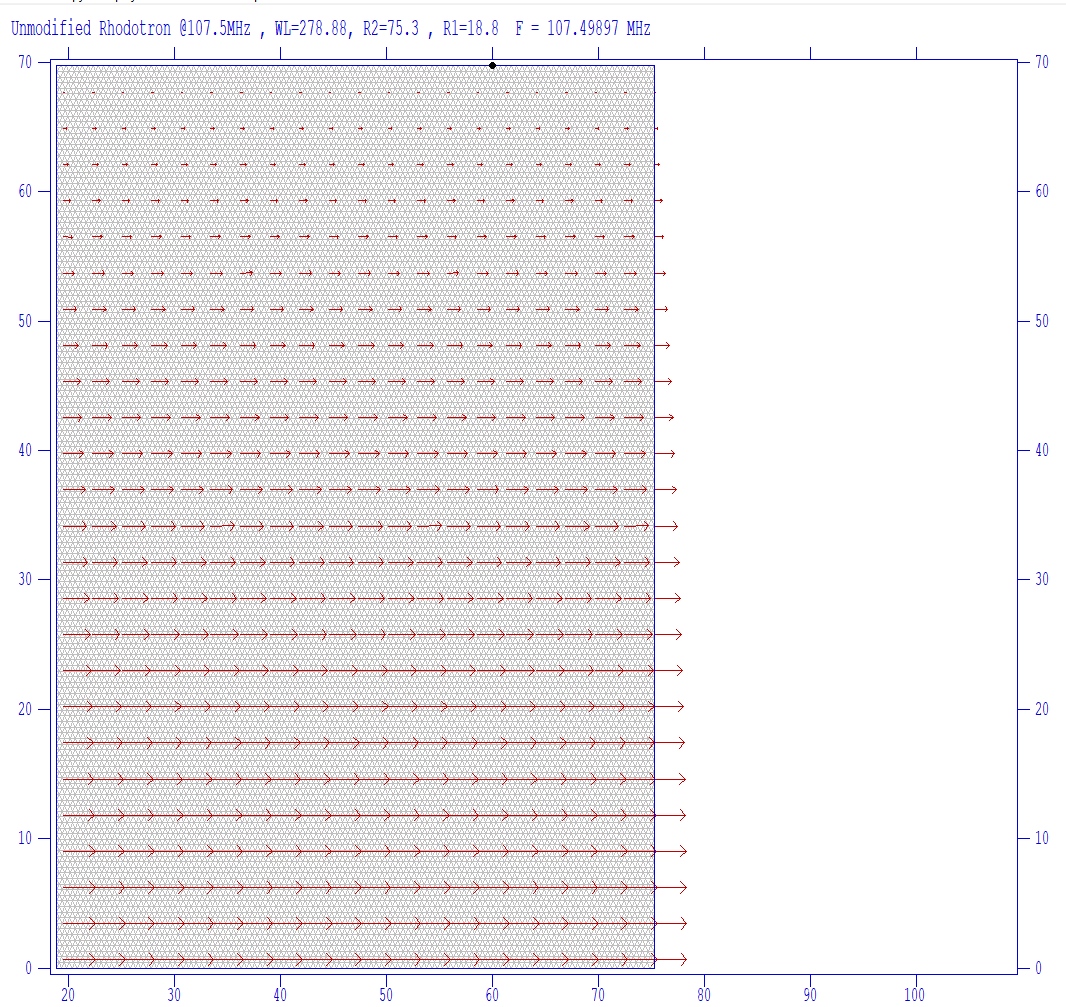
\includegraphics[width=\linewidth]{./figures/superfish/superfish107.png}
      \caption{107.5 MHz}
    \end{subfigure}%
    \centering
    \begin{subfigure}{.5\textwidth}
      \centering
      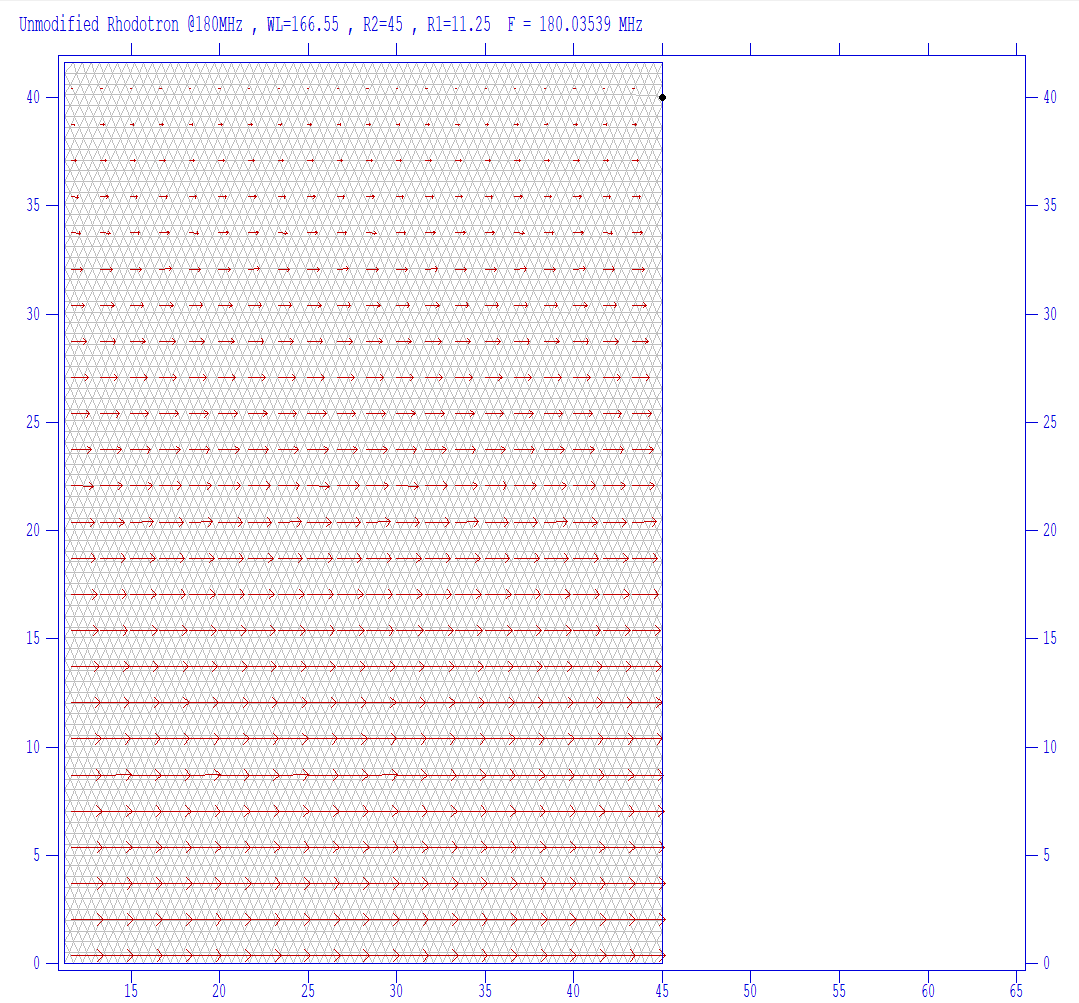
\includegraphics[width=\linewidth]{./figures/superfish/superfish180.png}
      \caption{180 MHz}
    \end{subfigure}
    \caption{Poission Superfish results for \fromeq{107_180_MHZ_cavity_design_parameters}}
    \label{fig:107_simple_cavity_design}
\end{figure}

\begin{figure}[H]
    \centering
    \begin{subfigure}{.5\textwidth}
      \centering
      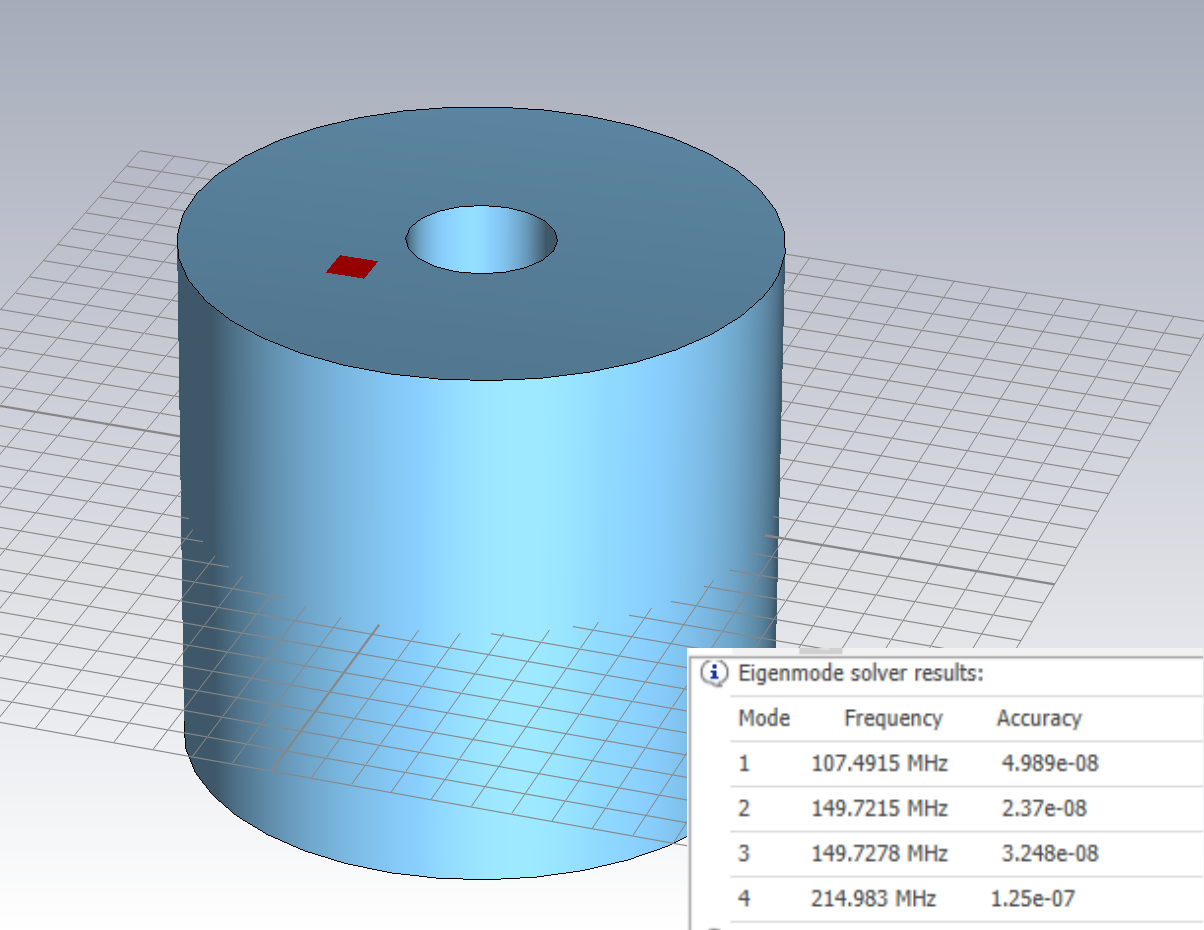
\includegraphics[width=\linewidth]{./figures/cst/cst107.png}
      \caption{107.5 MHz}
    \end{subfigure}%
    \begin{subfigure}{.5\textwidth}
      \centering
      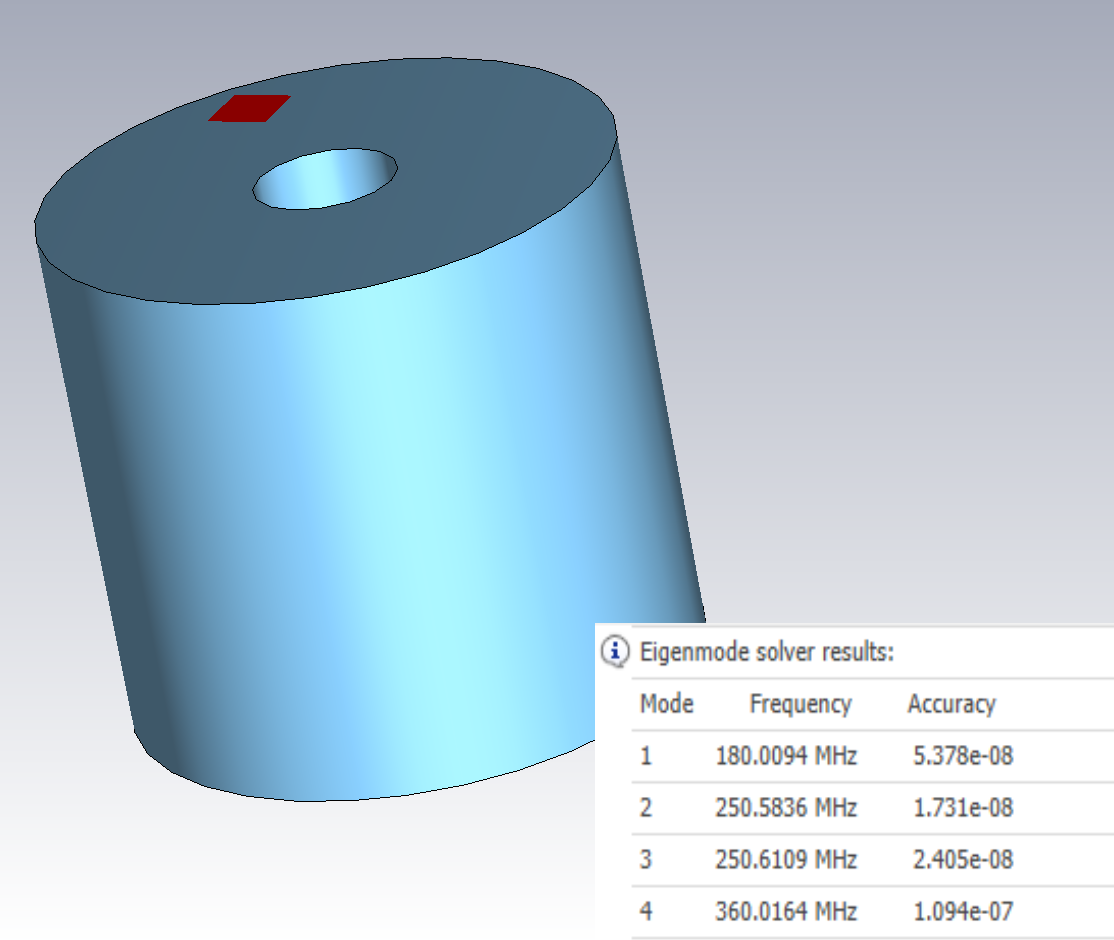
\includegraphics[width=.9\linewidth]{./figures/cst/cst180.png}
      \caption{180 MHz}
    \end{subfigure}
    \caption{CST Eigenmode results for \fromeq{107_180_MHZ_cavity_design_parameters}}
    \label{fig:180_simple_cavity_design}
\end{figure}

\begin{figure}[H]
    \centering
    \begin{subfigure}{.5\textwidth}
      \centering
      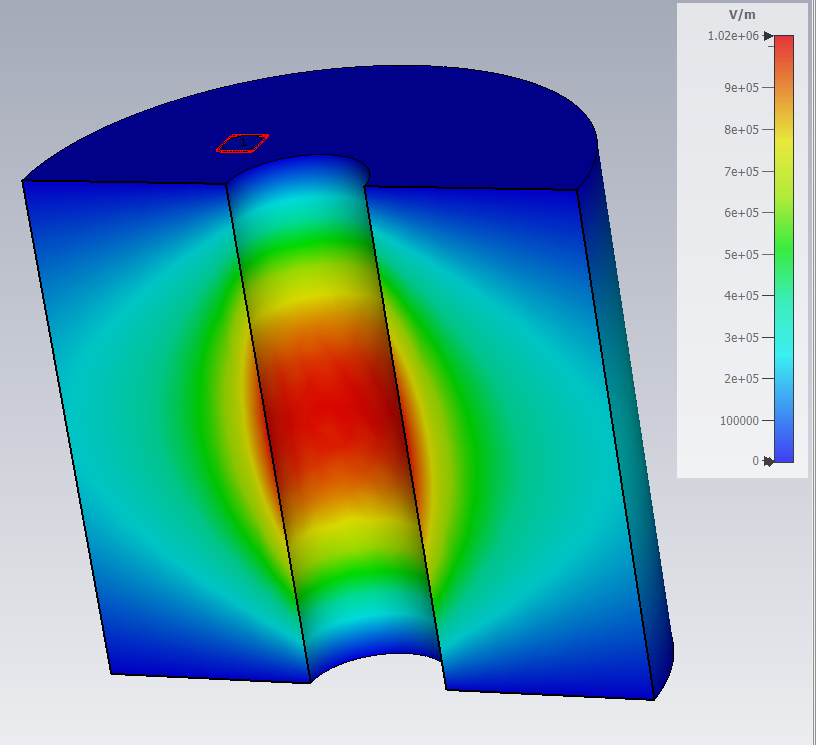
\includegraphics[width=.9\linewidth]{./figures/cst/cst107_e.png}
      \caption{107.5 MHz}
    \end{subfigure}%
    \begin{subfigure}{.5\textwidth}
      \centering
      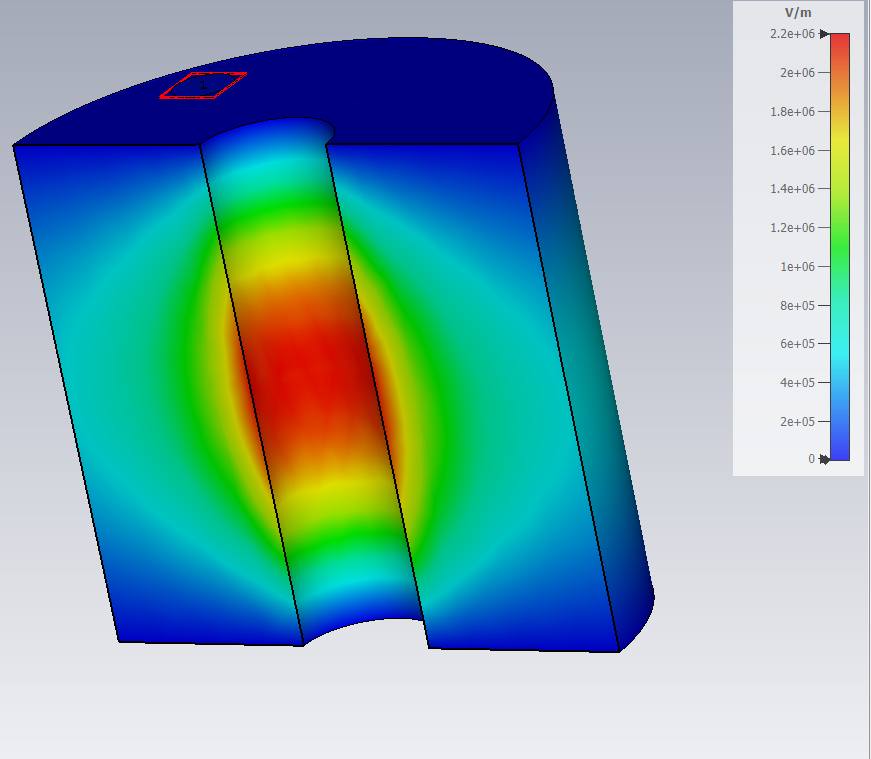
\includegraphics[width=.94\linewidth]{./figures/cst/cst180_e.png}
      \caption{180 MHz}
    \end{subfigure}
    \caption{CST Electric field solutions for \fromeq{107_180_MHZ_cavity_design_parameters}}
    \label{fig:cst_simple_cavity_designs}
\end{figure}




As mentioned by POTTIER, truncated cone terminations in inner cylinder can improve the shunt empedance $Z$ of the cavity \cite{rhodo_pottier}. 
Below, \textit{Poission superfish} results of such a modification with matching height increase to keep resonant frequency can be found.

\begin{figure}[H]
    \centering
    \begin{subfigure}{.5\textwidth}
      \centering
      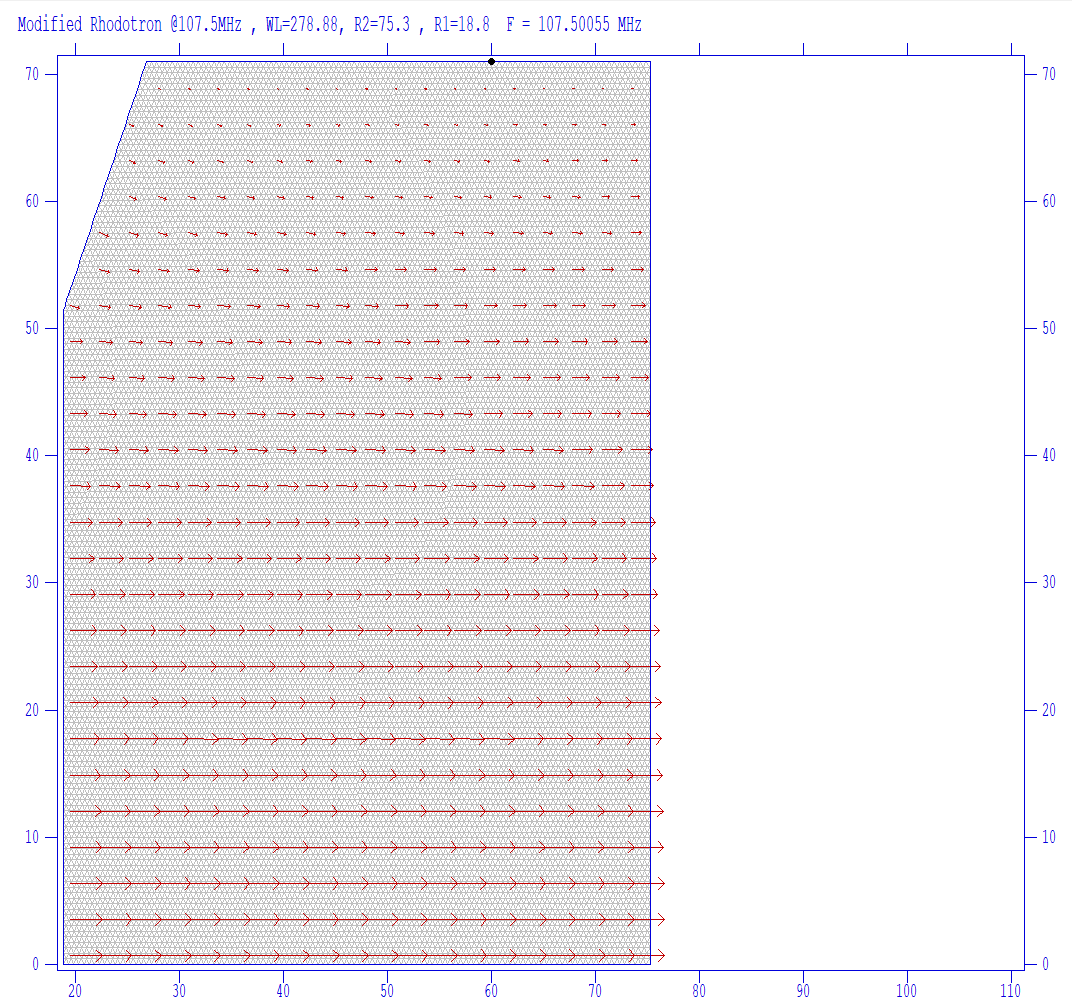
\includegraphics[width=.9\linewidth]{./figures/superfish/superfish107mod.png}
      \caption{107.5 MHz truncated}
    \end{subfigure}%
    \begin{subfigure}{.5\textwidth}
      \centering
      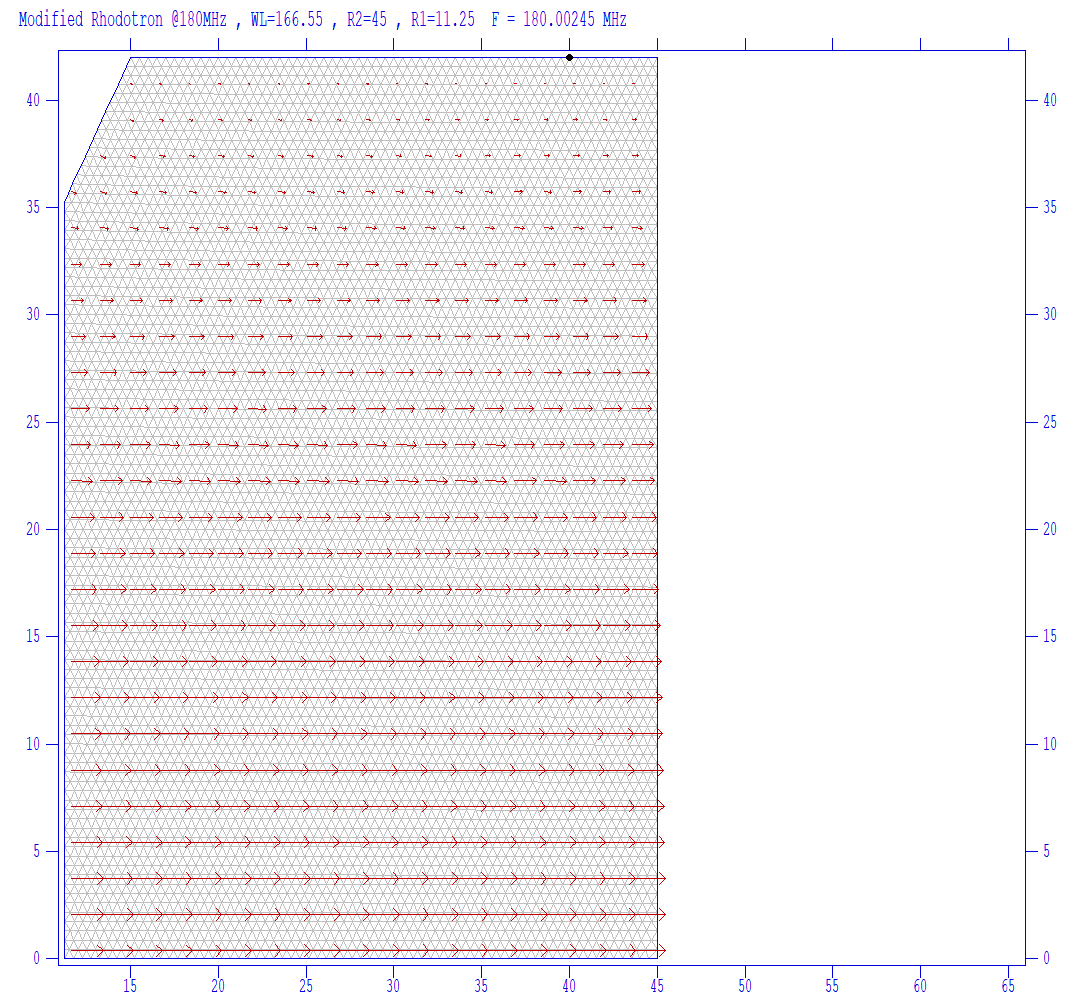
\includegraphics[width=.9\linewidth]{./figures/superfish/superfish180mod.png}
      \caption{180 MHz truncated}
    \end{subfigure}
    \caption{Poisson SUPERFISH field results of truncated cavities}
    \label{fig:107_180_modified_cavities_superfish}
\end{figure}

\begin{figure}[H]
    \centering
    \begin{subfigure}{.5\textwidth}
      \centering
      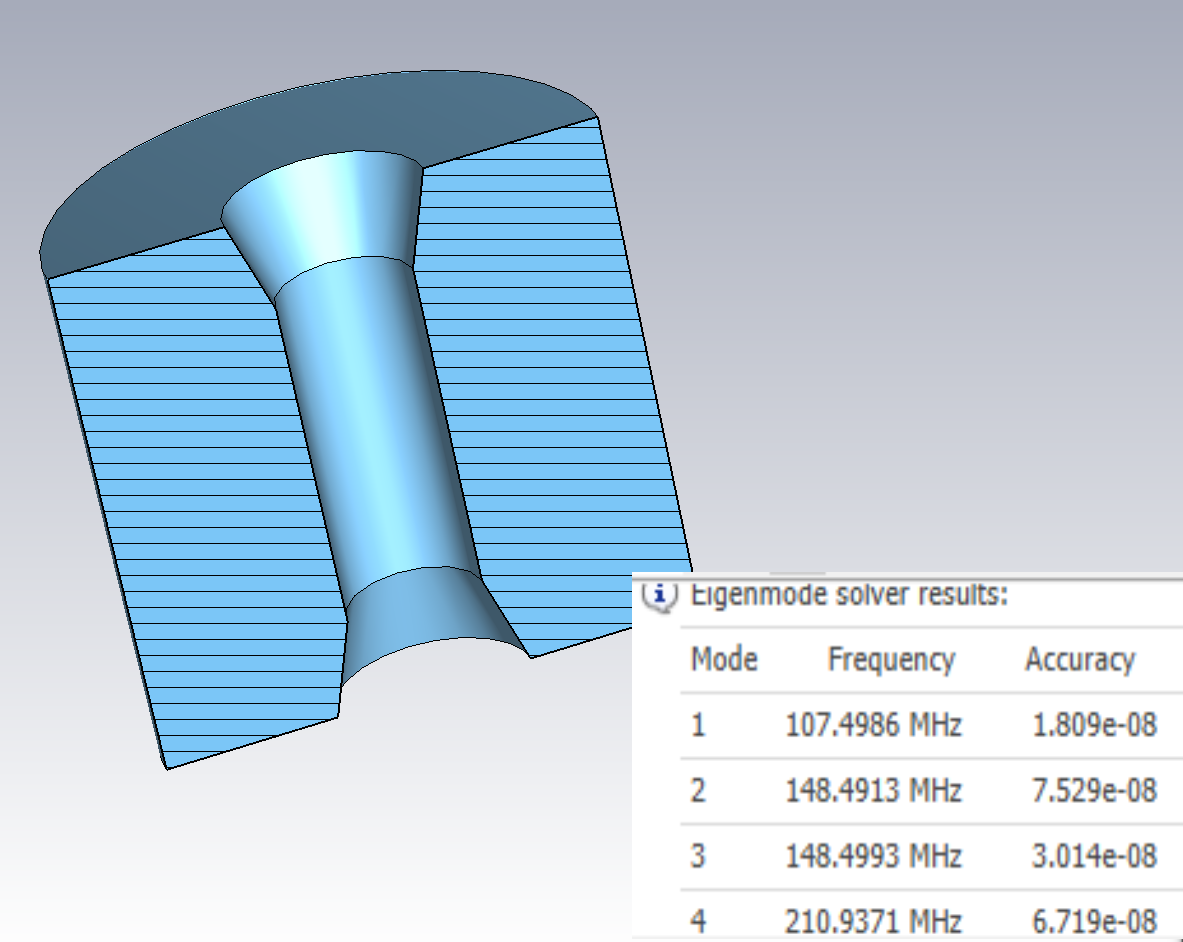
\includegraphics[width=.9\linewidth]{./figures/cst/cst107mod.png}
      \caption{107.5 MHz truncated}
    \end{subfigure}%
    \begin{subfigure}{.5\textwidth}
      \centering
      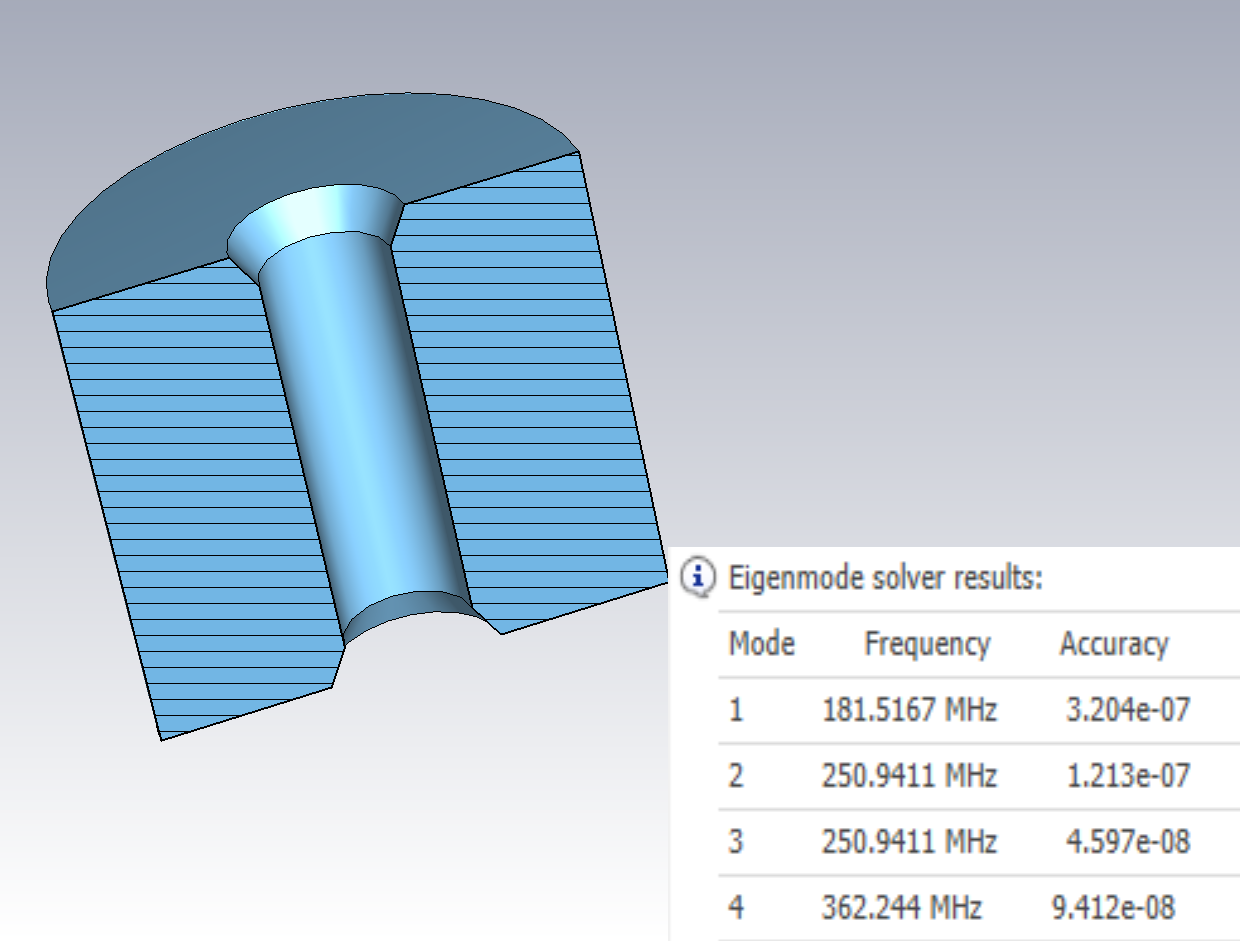
\includegraphics[width=.9\linewidth]{./figures/cst/cst180mod.png}
      \caption{180 MHz truncated}
    \end{subfigure}
    \caption{CST eigenmode results of truncated cavities}
    \label{fig:107_180_modified_cavities_cst_eigenmode}
\end{figure}

\begin{figure}[H]
    \centering
    \begin{subfigure}{.5\textwidth}
      \centering
      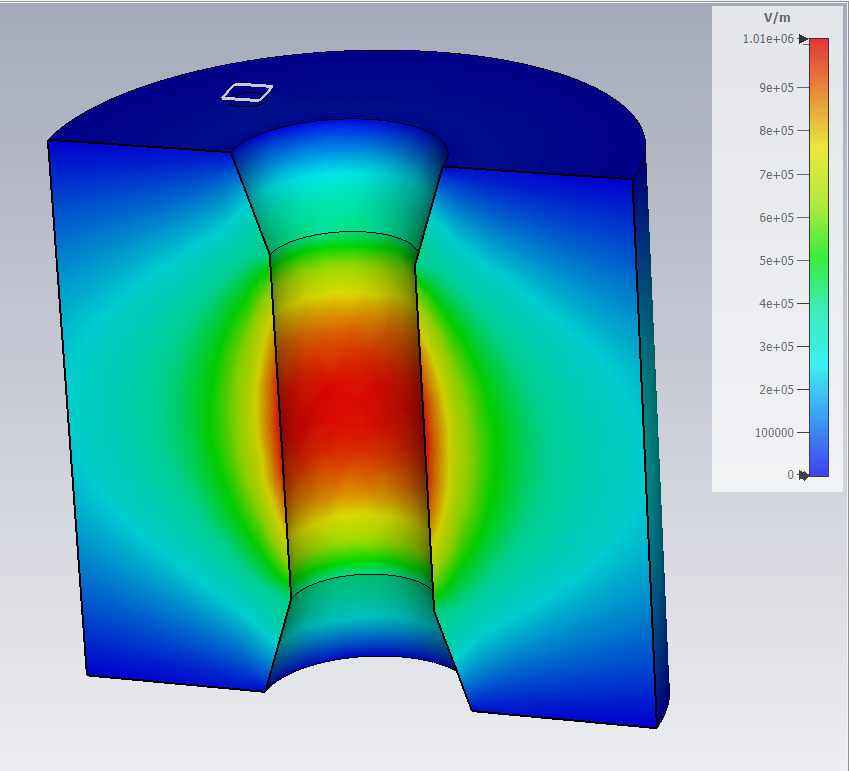
\includegraphics[width=.9\linewidth]{./figures/cst/cst107mod_e.png}
      \caption{107.5 MHz truncated}
    \end{subfigure}%
    \begin{subfigure}{.5\textwidth}
      \centering
      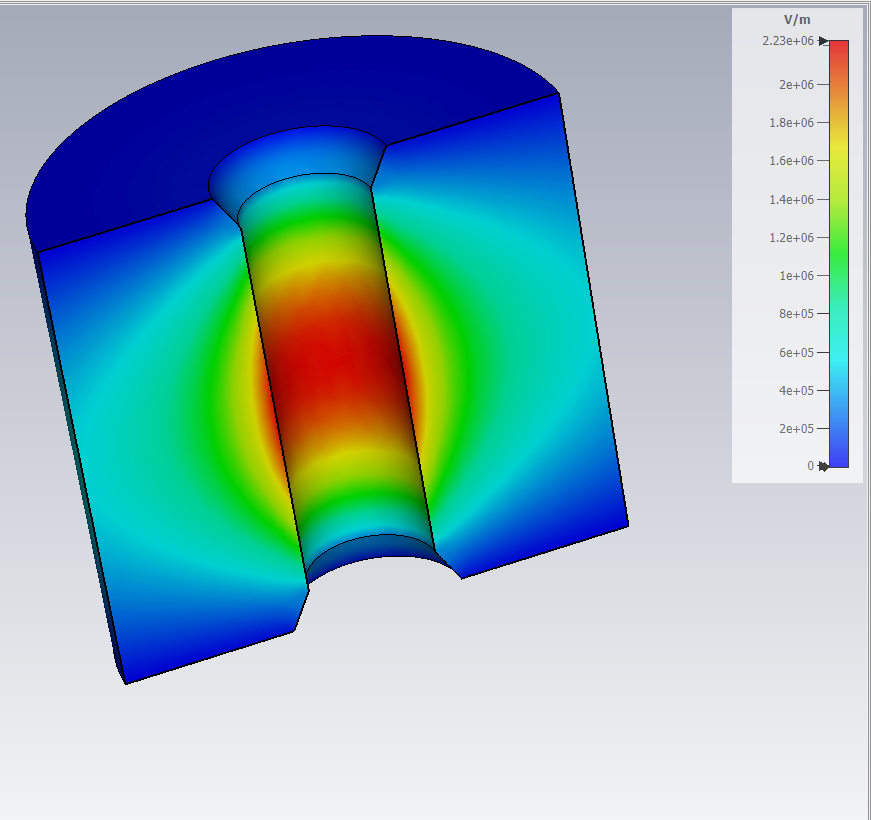
\includegraphics[width=.88\linewidth]{./figures/cst/cst180mod_e.png}
      \caption{180 MHz truncated}
    \end{subfigure}
    \caption{CST electric field results of truncated cavities}
    \label{fig:107_180_modified_cavities_cst_field}
\end{figure}

\begin{figure}[H]
    \centering
    \begin{subfigure}{.5\textwidth}
      \centering
      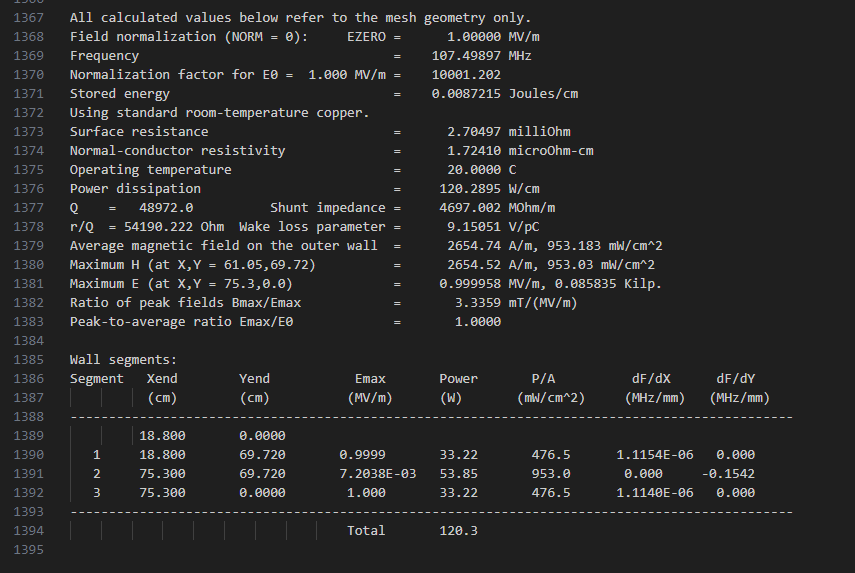
\includegraphics[width=0.97\linewidth]{./figures/superfish/superfish107_z.png}
      \caption{107.5 MHz unmodified}
    \end{subfigure}%
    \begin{subfigure}{.5\textwidth}
      \centering
      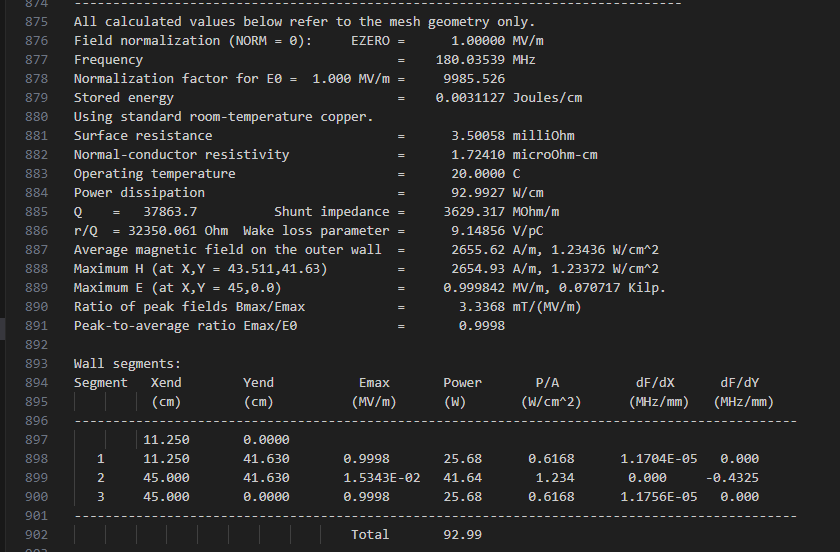
\includegraphics[width=0.99\linewidth]{./figures/superfish/superfish180_z}
      \caption{180 MHz unmodified}
    \end{subfigure}
    \caption{Poisson Superfish calculations with \textit{unmodified} cavities}
    \label{fig:107_cavity_shunt_diff}
\end{figure}
    
\begin{figure}[H]
    \centering
    \begin{subfigure}{.5\textwidth}
      \centering
      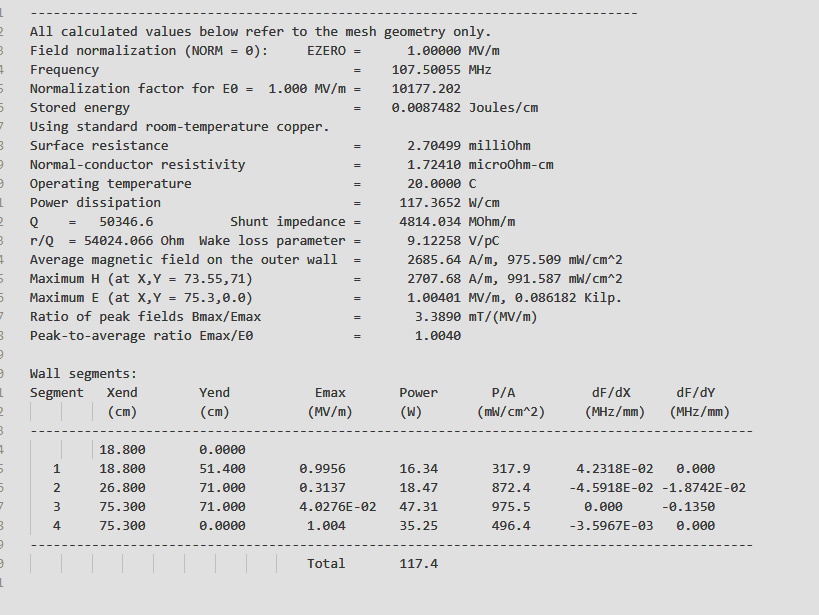
\includegraphics[width=0.95\linewidth]{./figures/superfish/superfish107mod_z.png}
      \caption{107.5 MHz truncated}
    \end{subfigure}%
    \begin{subfigure}{.5\textwidth}
      \centering
      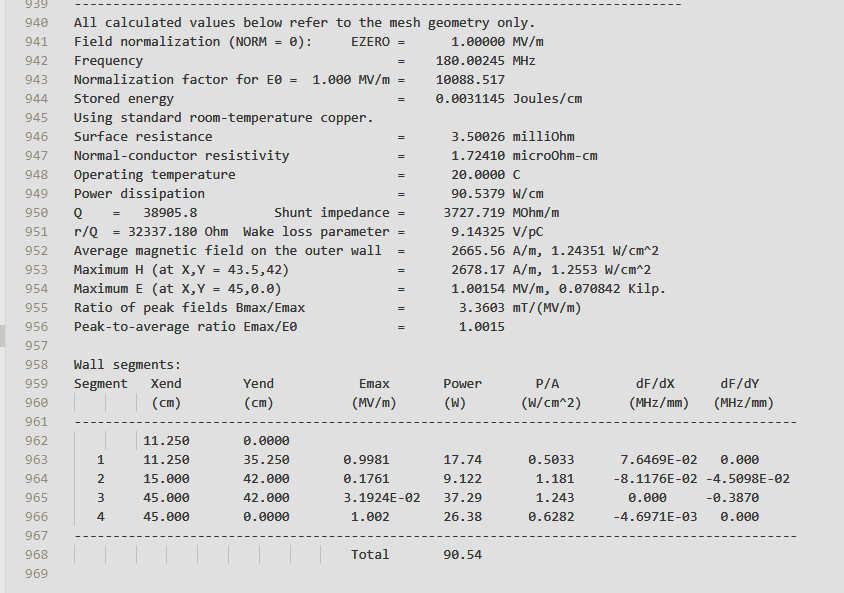
\includegraphics[width=\linewidth]{./figures/superfish/superfish180mod_z.png}
      \caption{180 MHz truncated}
    \end{subfigure}
    \caption{Poisson Superfish calculations with \textit{truncated} cavities}
    \label{fig:180_cavity_shunt_diff}
\end{figure}
    

One can observe the shunt impedance gain between truncated and unmodified cavities in \fromfigs{107_cavity_shunt_diff}{180_cavity_shunt_diff};
\begin{equation*}
    \begin{aligned}
        \Delta Z_{107.5}=2.5\%
    \end{aligned}
    \qquad
    \begin{aligned}
        \Delta Z_{180}=2.7\%
    \end{aligned}
\end{equation*}




\newpage



\section{Magnet Design} \label{sec:magnet_design}
Magnet design in rhodotron type accelerators depend heavily on the design of the cavities.
Because the limiting factors usually are frequency and total volume of the accelerator, magnet design parameters are considered after cavity design has been completed.
Considering the nature of coaxial cavity, simplest path for beams inside magnets is major segment of a circle, which was used as the reference for following discussions.

\begin{figure}[H]
    \captionsetup[subfigure]{justification=centering}
    \captionsetup{justification=centering}
    \centering
    \begin{subfigure}{.5\textwidth}
      \centering
      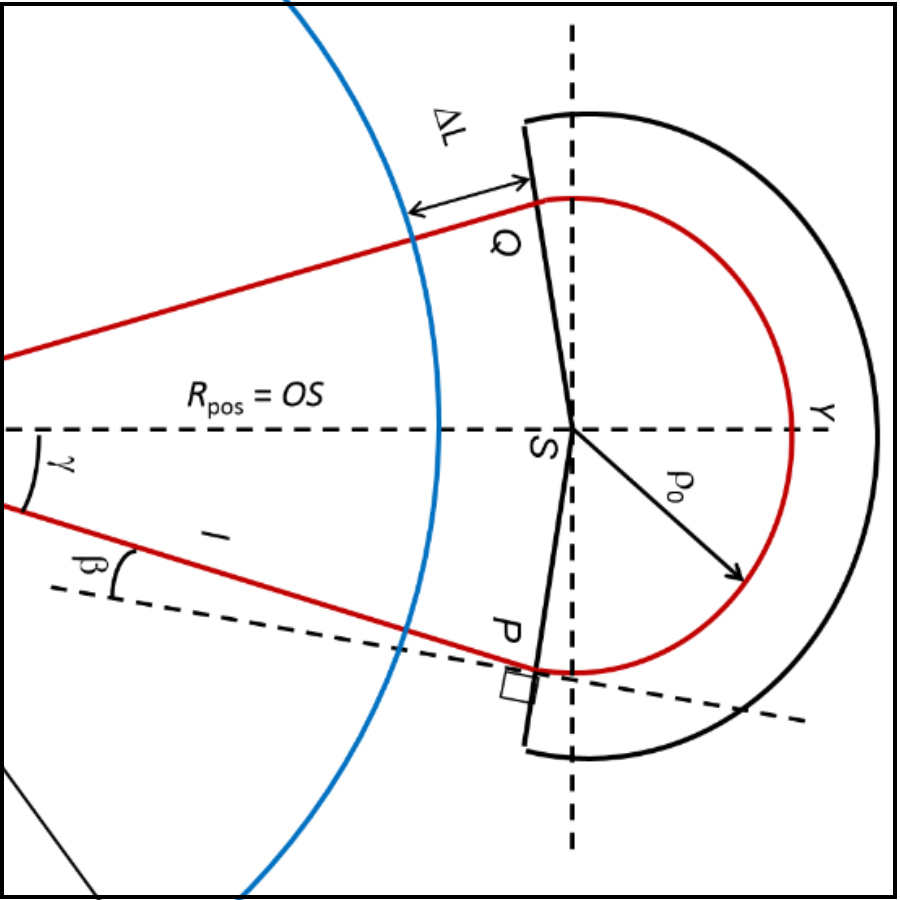
\includegraphics[width=.9\linewidth]{./figures/design/Ltot.png}
      \caption{Geometry of the outside trajectory \\ of a rhodotron \cite{cite:rhodo_design}}
    \end{subfigure}%
    \centering
    \begin{subfigure}{.5\textwidth}
      \centering
      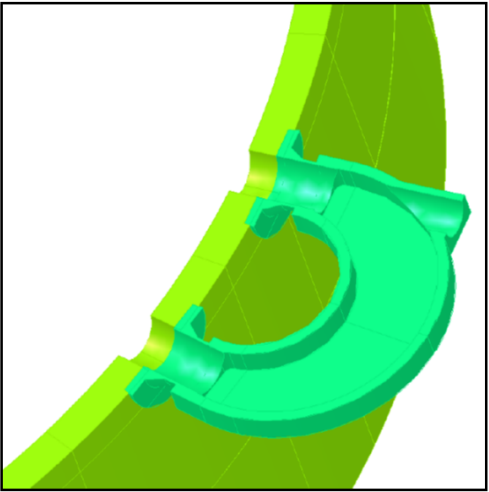
\includegraphics[width=.9\linewidth]{./figures/design/tt300_mag.png}
      \caption{Modeling of the outside trajectory \\ of a rhodotron (TT300) \cite{cite:rhodo_design}}
    \end{subfigure}
    \caption{From "Design and Simulation Tools for the \\ High-Intensity Industrial Rhodotron Electron Accelerator," \\by W.Kleeven, M.Abs, J.Brison, E.Forton, J.Hubert and J.Van de Walle}
    \label{fig:magnet_design_illustrations}
\end{figure}

In rhodotron accelerators, magnets are used for not only guiding the electron beam to desired path, but also for syncronizing them with the RF field in the cavity. 
This syncronization, also called phase stability, is the fundamental constraint of magnet design. 
Time spent outside of the cavity should be precisely tuned to maximize acceleration in the succeeding pass. 

Two different approaches have been used to achieve phase stability.
These approaches are discussed further in the following sections.

\subsection{$n\lambda$ Technique} \label{sec:n_L_technique}

First approach for phase stability considiration assumes that from the start of the current pass, $\beta_{avg} \approx 1$ for a synchronous particle. 

To maintain the phase synchronization, a particle that started the current pass at $t=0$, should start the next pass at $t=nT$, where $n$ is an integer and $T$ is the period of RF field inside cavity.
As discussed earlier, by assuming the electron is traveling at $c$, phase stability can be achieved by designing the whole trajectory to be $n \lambda$, where $\lambda$ is the wavelength of the RF field. 
In other words, total trajectory of synchronous particle needs to satisfy the following equality;
\begin{equation*}
    L_{pass} = n \lambda
\end{equation*} 
Since $n>1$ would require unnecessarily long and expensive beam guide and magnets, $n=1$ is the most efficient choice.
\begin{equation}
    L_{pass} = \lambda
\end{equation} 

\begin{figure}[H]    
    \centering
    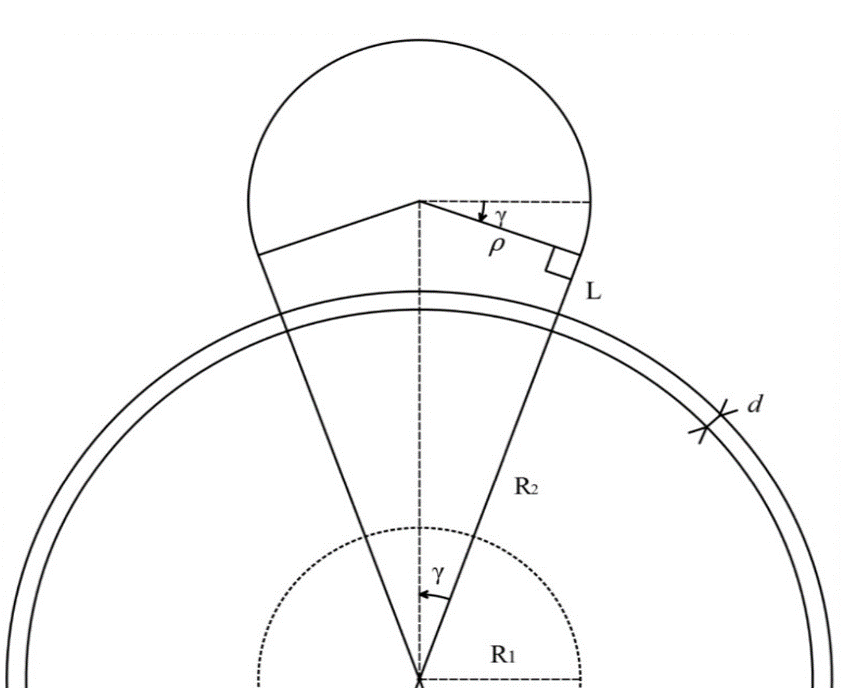
\includegraphics[width=.8\linewidth]{./figures/design/magnet_design.png}
    \caption{Trejectory of a particle in single pass}
    \label{fig:magnet_design}
\end{figure}

From \fromfig{magnet_design}, where $\gamma$ is half the angle between trajectories of successive passes, $\rho$ is the radius of the circular path inside magnet, $L$ is the length of the magnet guide, $d$ is the thickness of the cavity wall;
\begin{eqnarray}
    L_{in} &=& 2R_2 \nonumber\\
    L_{out} &=& 2L + 2d + (\pi + 2\gamma)\rho \nonumber \\
    L_{pass} &=& L_{in} + L_{out}  \nonumber \\
    \lambda &=& 2R_2 + 2d + 2L + (\pi + 2\gamma)\rho \label{eq:magnet_lambda_constraint}
\end{eqnarray}

After the cavity design is complete, only $L$, $\gamma$ and $\rho$ remain, which are the design parameters of magnets.
Observing the \fromfig{magnet_design} and using \fromeq{magnet_lambda_constraint},

\begin{eqnarray}
    tan(\gamma) &=& \frac{\rho}{R_2 + d + L} \nonumber \\
    \rho &=&  tan(\gamma) (R_2 + d + L) \nonumber\\
    2\rho &=& tan(\gamma) (\lambda - (\pi + 2\gamma)\rho) \nonumber\\
    \rho (2 + tan(\gamma)(\pi + 2\gamma)) &=&  tan(\gamma) \lambda \nonumber\\
    \rho &=& \frac{\lambda}{\pi + 2\gamma + \frac{2}{tan(\gamma)}} \label{eq:magnet_rho_constraint} \\
    L + d &=& \frac{\rho}{tan(\gamma)} - R_2 \label{eq:magnet_L_constraint}
\end{eqnarray}

\textit{Equations \ref{eq:magnet_rho_constraint} and \ref{eq:magnet_L_constraint}} define 2 constraints. As already discussed, it has been assumed that cavity design is set (\textit{i.e} $R_2$, $\lambda$, $d$ are already defined).
Therefore only the magnet design parameters $\rho$, $\gamma$ and $L$ are left. Together with the constraints, one free variable defines the whole magnet design. 
Considering the importance of $\gamma$ for maximum number of possible passes, it will be used as the free magnet design variable in the further discussions.


\subsection{$L_{out}$ Parameter Sweep} \label{sec:parameter_sweep}

As mentioned previously in \fromsec{n_L_technique}, \fromeq{magnet_lambda_constraint} assumes that the particles are fast enough so that $\Delta t_{pass} \approx n T$. 
This assumption is not guaranteed however, especially in the first few passes if the particles are not accelerated enough. 
This scenario can happen when RF power is not sufficiently high. 

Consider an RF supply with $f=1$ GHz, $P=50$ kW. Using \fromeq{W_total_gain_pottier}, 
after the first pass the synchronous electron that entered the accelerator with $40$ keV and $\phi=15^\circ$ phase lag,
\begin{eqnarray*}
    W_{gain} &=& 2.14\times0.2998^{1/4}\times 50000^{1/2} = 354keV \\
    W_{total} &=& 394 keV \\
    \beta_{40keV} &\approx& 0.374 \\
    \beta_{394keV} &\approx& 0.825
\end{eqnarray*}
It is clear that $\beta_{avg}$ is not fast enough to sustain phase stability if the magnet is designed for $\beta = 1$. 
For these cases, \fromeq{magnet_lambda_constraint} fails to deliver phase stability.
Another approach for designing a magnet would be to find a new constraint, $K$ for total path length.
\begin{eqnarray*}
    L_{pass} &=& K \\
    L_{in} + L_{out} &=& K
\end{eqnarray*}

Since $L_{in}$ is set previously from cavity design, we can remove it from our equation and continue with
\begin{equation} \label{eq:mag_sweep_constraint}
    L_{out} = K
\end{equation}

To start, an optimization criteria for the following pass such as
\begin{itemize}
    \item Ensure the phase stability of the synchronous electron
    \item Maximize the energy gain of the synchronous electron
    \item Minimize the energy spread of the beam
    \item Minimize the phase lag spread of the beam
    \item All of the above with decided weights
\end{itemize}
needs be selected. Using a simulation software such as \textit{CST Studio Particle Module}, the optimum value of $K$ for the criteria can be found by simulating for different values of $K$ (\textit{sweeping}) and analyzing the results.
This process can be repeated for each magnet until the desired beam characteristics in the end of the accelerator are achieved.

However, one caviat of this technique is that, available simulation softwares are not well suited for this kind of process. As mentioned above, \textit{CST Studio Particle Module} has a \textit{parameter sweep} functionality.
But the calculation times are too slow to be useful in this particular problem. \textit{A custom built software offering magnet optimizing sweep functionality will be discussed in the following chapter.}



\newpage



\section{Initial Design at KAHVELab} 

A rhodotron with operation frequency of $107.5$ MHz was decided to be built at KAHVELab. 
After considering the earlier simulations mentioned in \fromsecs{cavity_design}{magnet_design}, an initial design was created.

\begin{figure}[H]
    \centering
    \captionsetup{justification=centering}
    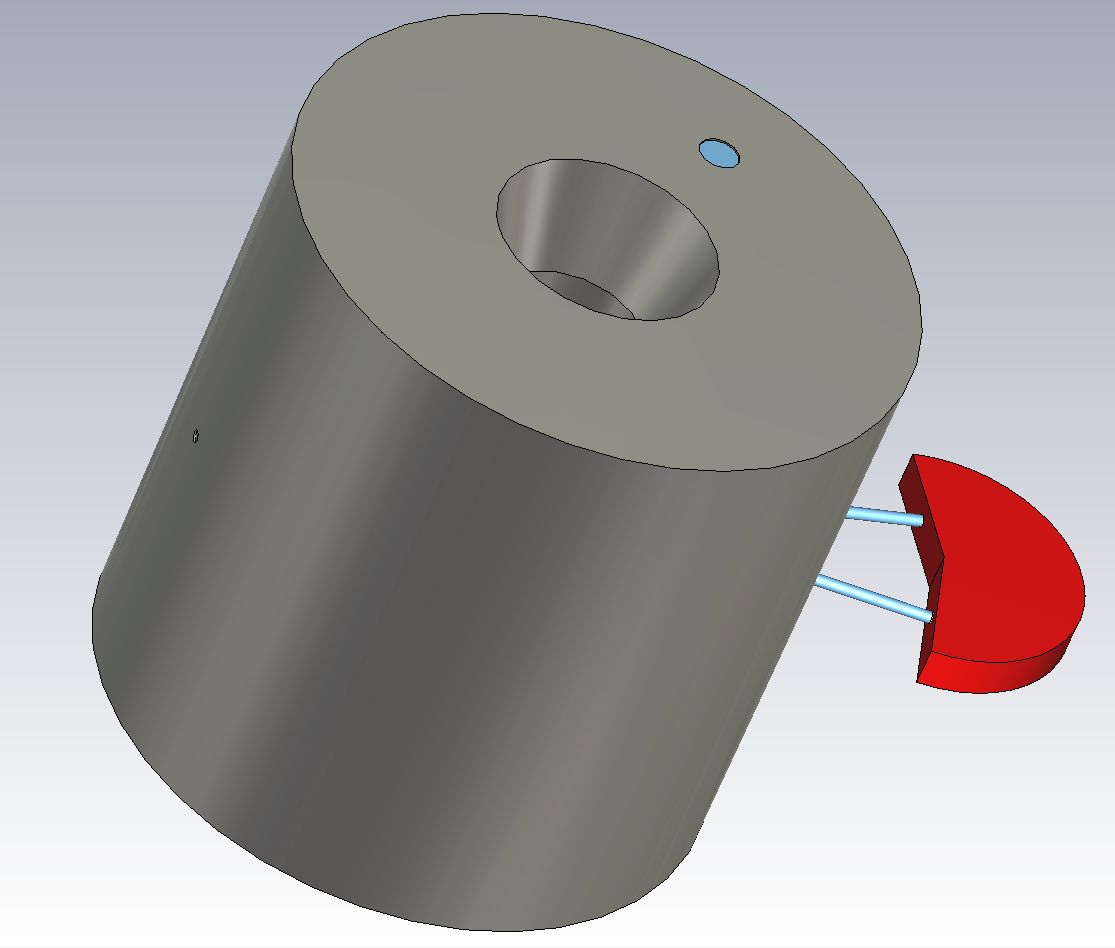
\includegraphics[width=.5\linewidth]{./figures/cst/cst_first_design1.png}
    \caption{Initial design of the proposed rhodotron \\ $\gamma=9^\circ$}
    \label{fig:initial_design}
\end{figure}
\begin{figure}[H]
    \captionsetup[subfigure]{justification=centering}
    \captionsetup{justification=centering}
    \centering
    \begin{subfigure}{.5\textwidth}
      \centering
      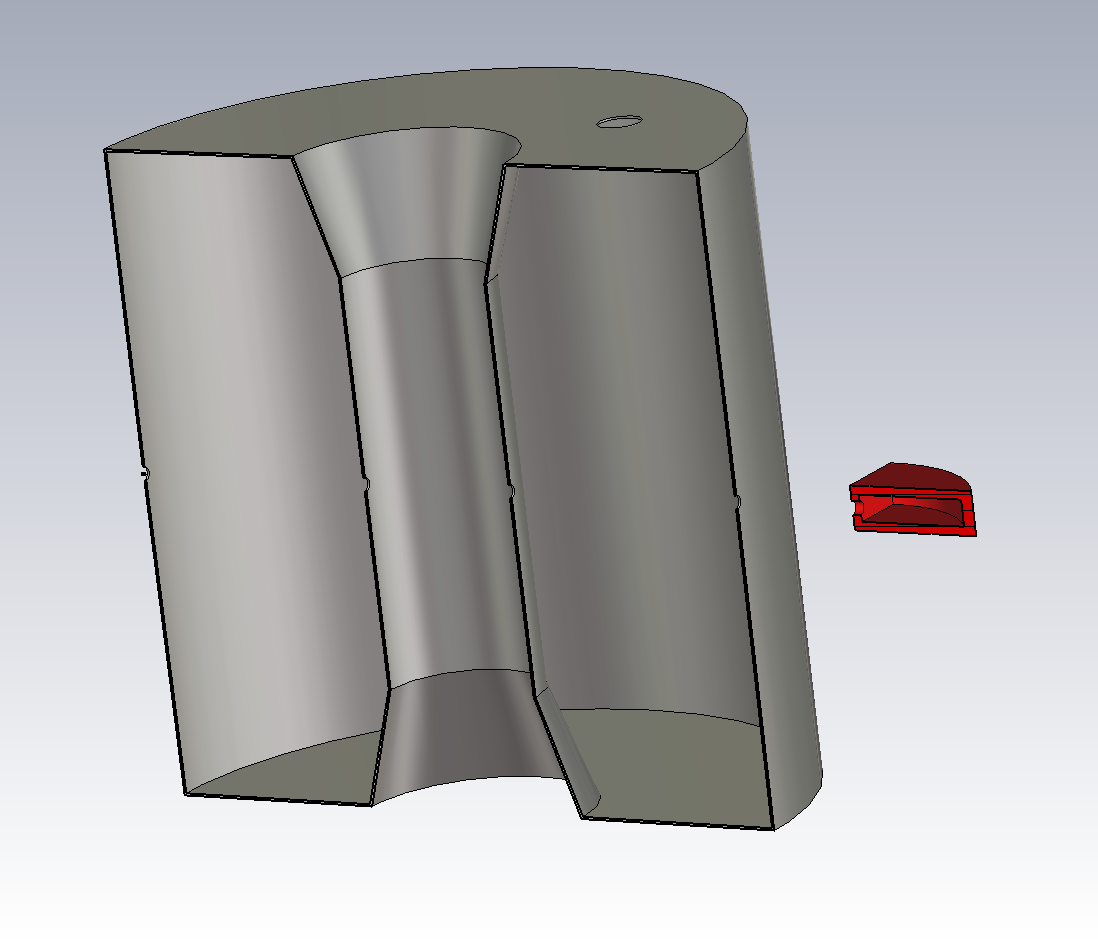
\includegraphics[width=.92\linewidth]{./figures/cst/cst_first_design3.png}
      \caption{Axial cross section.}
    \end{subfigure}%
    \centering
    \begin{subfigure}{.5\textwidth}
      \centering
      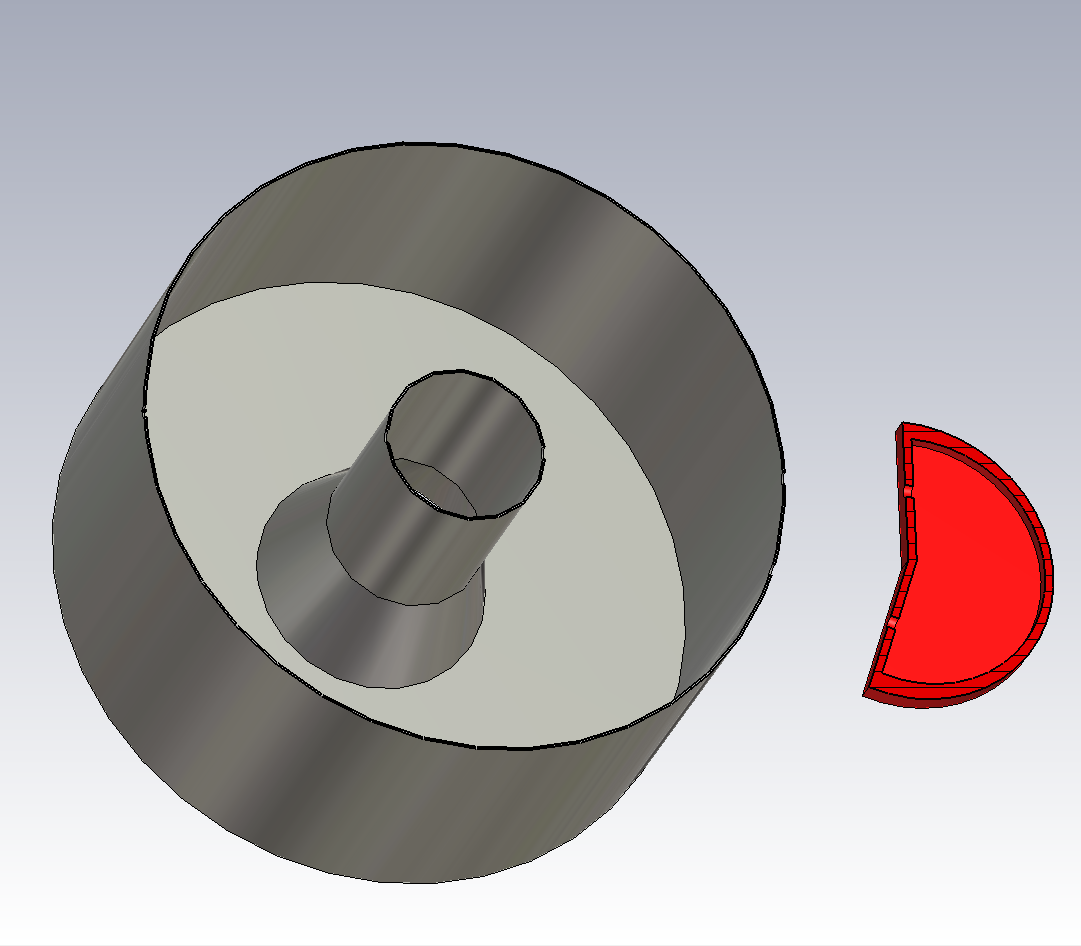
\includegraphics[width=.9\linewidth]{./figures/cst/cst_first_design2.png}
      \caption{Cross section at acceleration plane.}
    \end{subfigure}
    \caption{Initial design of the proposed rhodotron.}
    \label{fig:initial_design_cross_section}
\end{figure}
The magnets used in this design is the simplest in terms of design parameters. It consists of an iron casing encapsulating the shape of desired magnetic field, which are created by two coils inside.

\begin{figure}[H]
    \captionsetup[subfigure]{justification=centering}
    \captionsetup{justification=centering}
    \centering
    \begin{subfigure}{.5\textwidth}
      \centering
      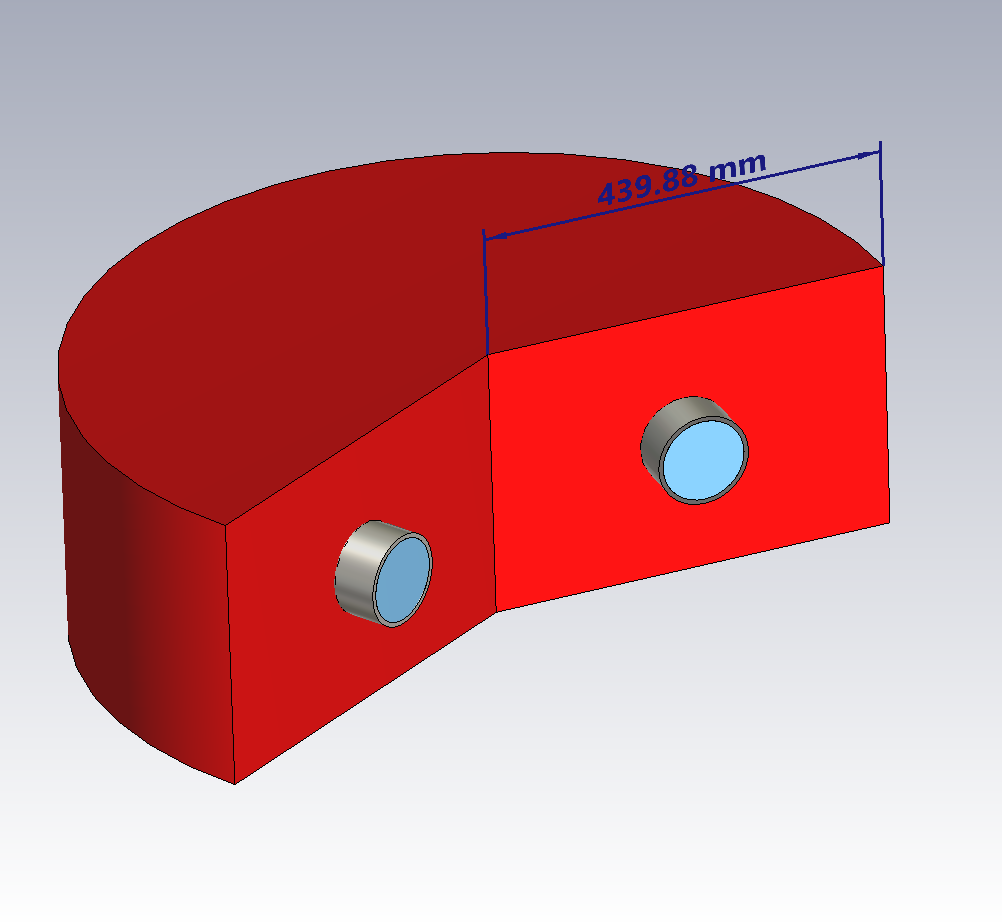
\includegraphics[width=.9\linewidth]{./figures/cst/cst_first_magnet_design1.png}
    \end{subfigure}%
    \centering
    \begin{subfigure}{.5\textwidth}
      \centering
      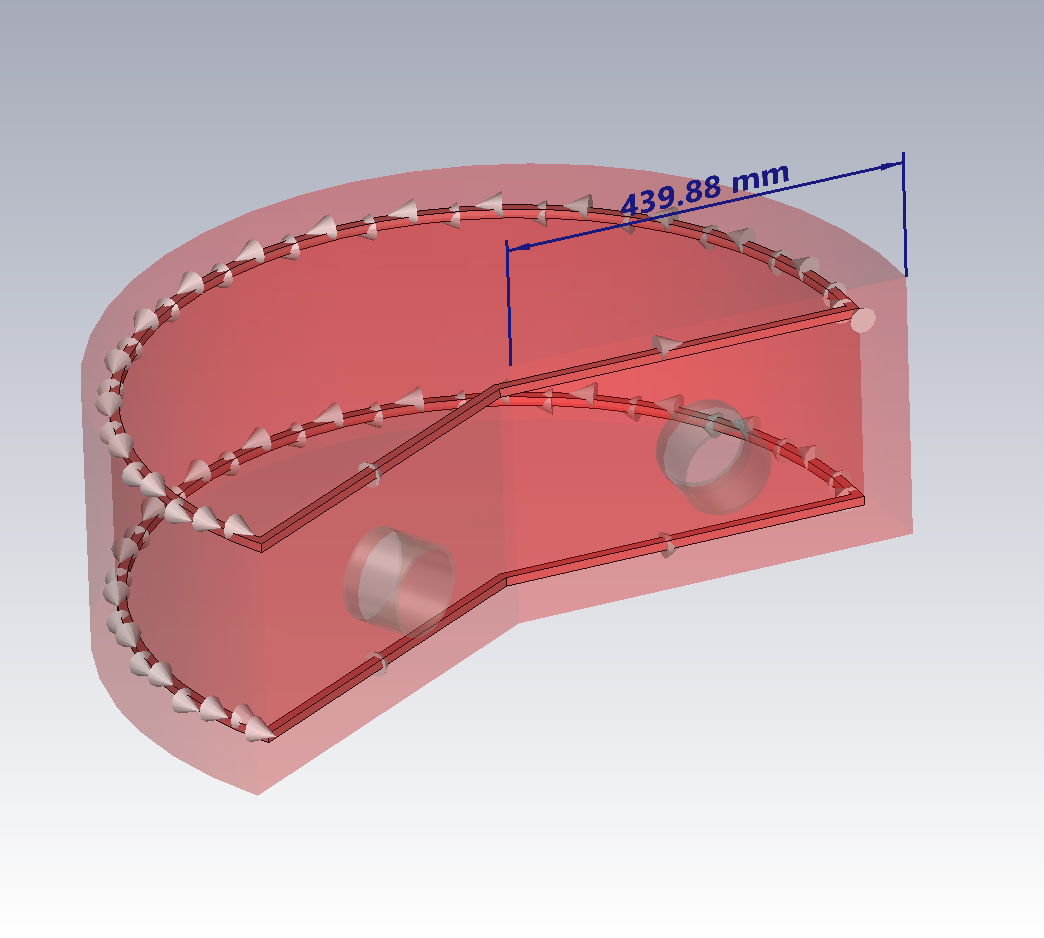
\includegraphics[width=.92\linewidth]{./figures/cst/cst_first_magnet_design2.png}
    \end{subfigure}
    \caption{Initial magnet design.}
    \label{fig:initial_magnet_design}
\end{figure}

\begin{figure}[H]
    \centering
    \captionsetup{justification=centering}
    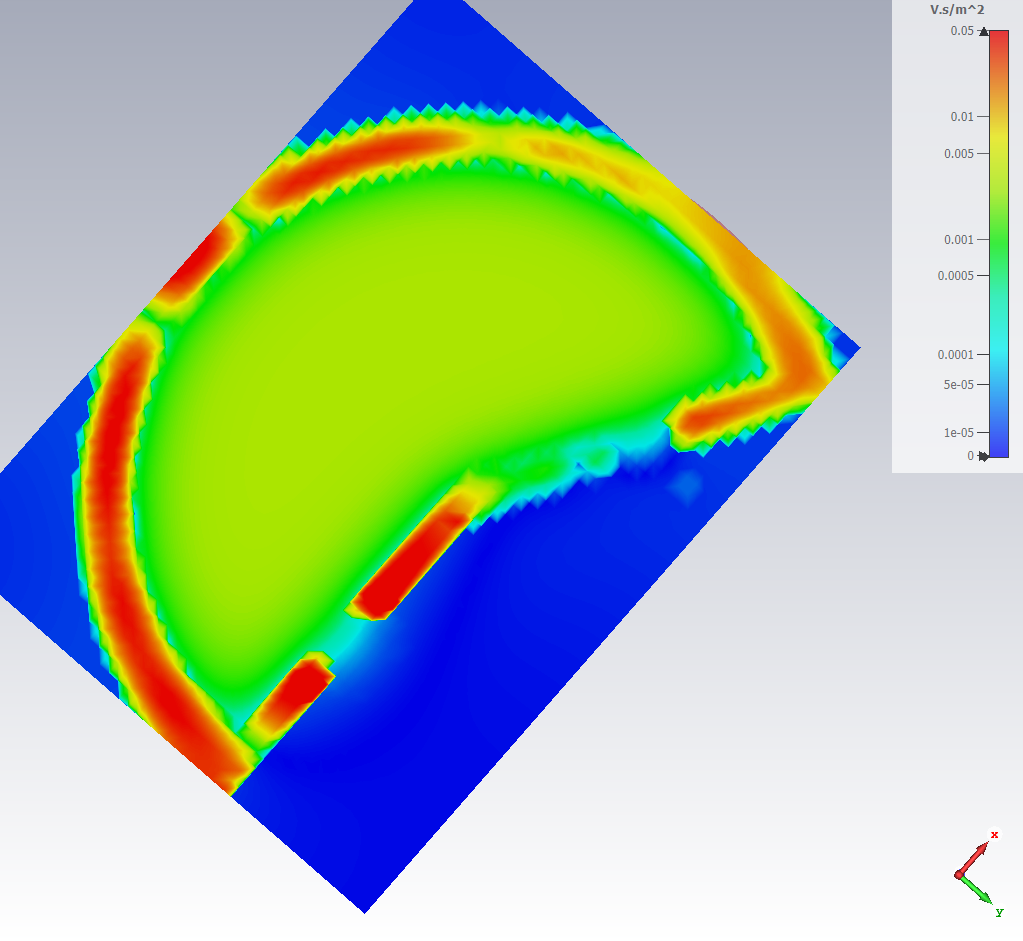
\includegraphics[width=.8\linewidth]{./figures/cst/cst_first_magnet_design3.png}
    \caption{Magnetic field in acceleration plate of initial magnet design.}
    \label{fig:initial_magnet_design_B}
\end{figure}

\fromfig{initial_magnet_design_B} shows that this design provides relatively uniform magnetic field inside, although magnetic field gradient in the openings can be improved. 

After adding two more magnets and using $\gamma=15^\circ$, the following second prototype design was created

\begin{figure}[H]
    \centering
    \captionsetup{justification=centering}
    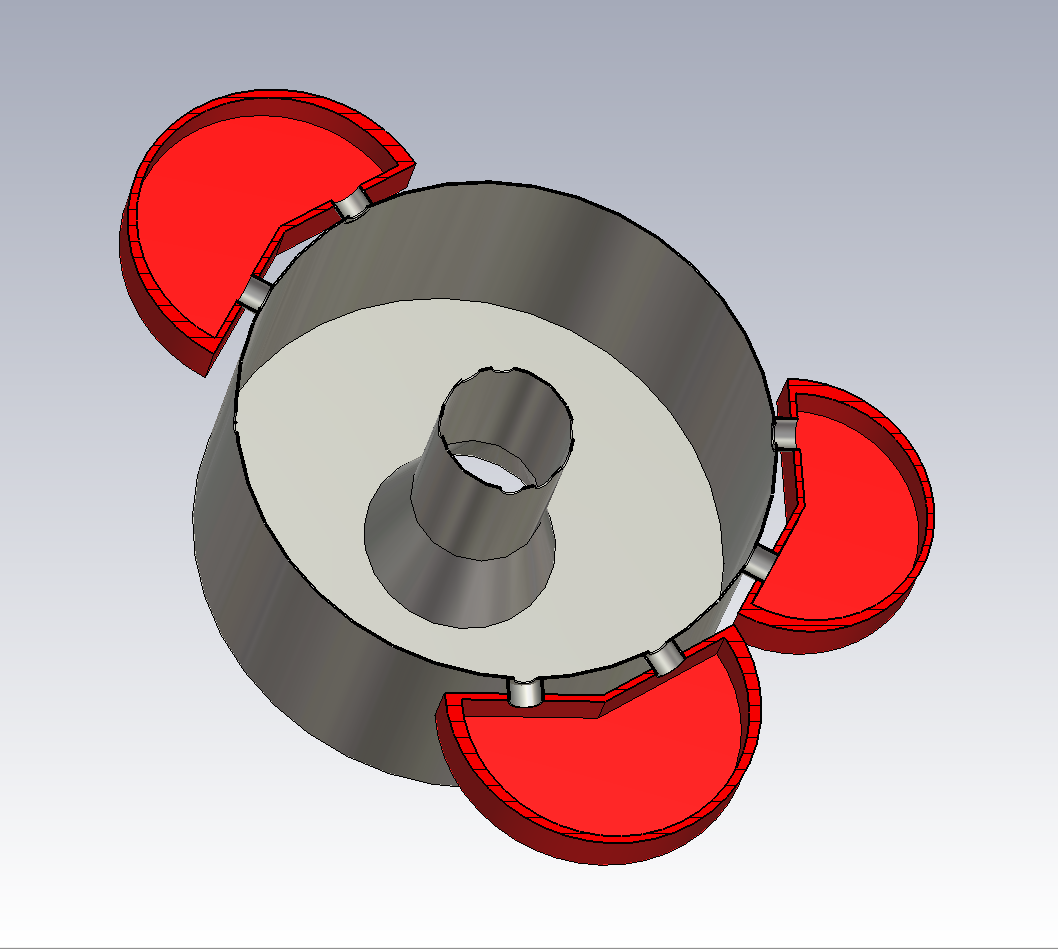
\includegraphics[width=.8\linewidth]{./figures/cst/cst_second_design2.png}
    \caption{Initial cavity with three magnets as shown in \fromfig{initial_magnet_design} \\ $\gamma=15^\circ$}
    \label{fig:initial_three_magnet_design}
\end{figure}

These designs, together with $40$ keV $e^-$ gun injecting with phase lag of $15^\circ$ for $0.1$ ns, was simulated at RF power of $12$ kW using \textit{CST Studio Particle Module PIC Solver}.
Results of these simulations can be found in \fromfig{initial_designs_PIC_phase_space_monitor}.

\begin{figure}[H]
    \captionsetup[subfigure]{justification=centering}
    \captionsetup{justification=centering}
    \centering
    \begin{subfigure}[b]{.8\textwidth}
      \centering
      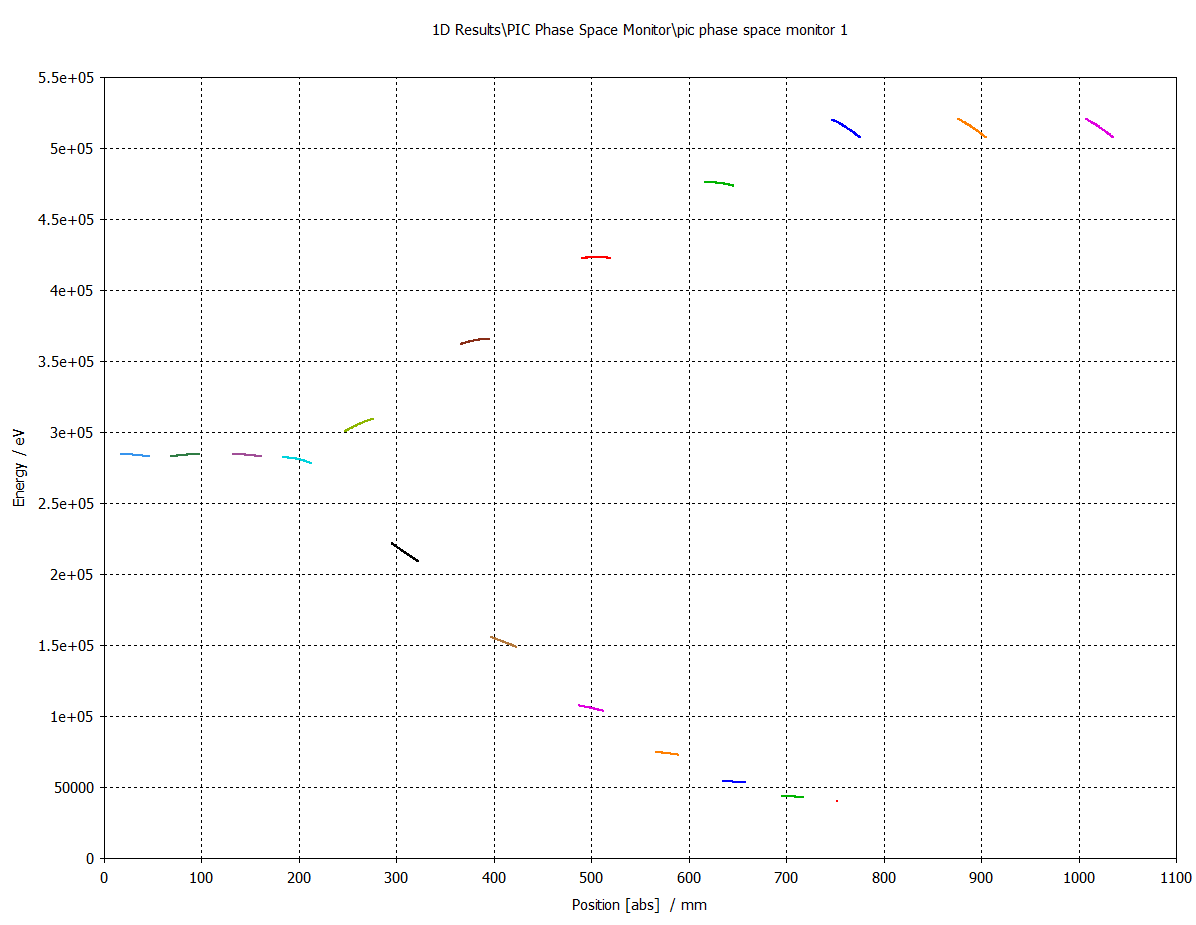
\includegraphics[width=\linewidth]{./figures/cst/cst_first_design4.png}
      \caption{One pass simulation of \fromfig{initial_design}}
    \end{subfigure}
    \centering
    \begin{subfigure}[b]{.8\textwidth}
      \centering
      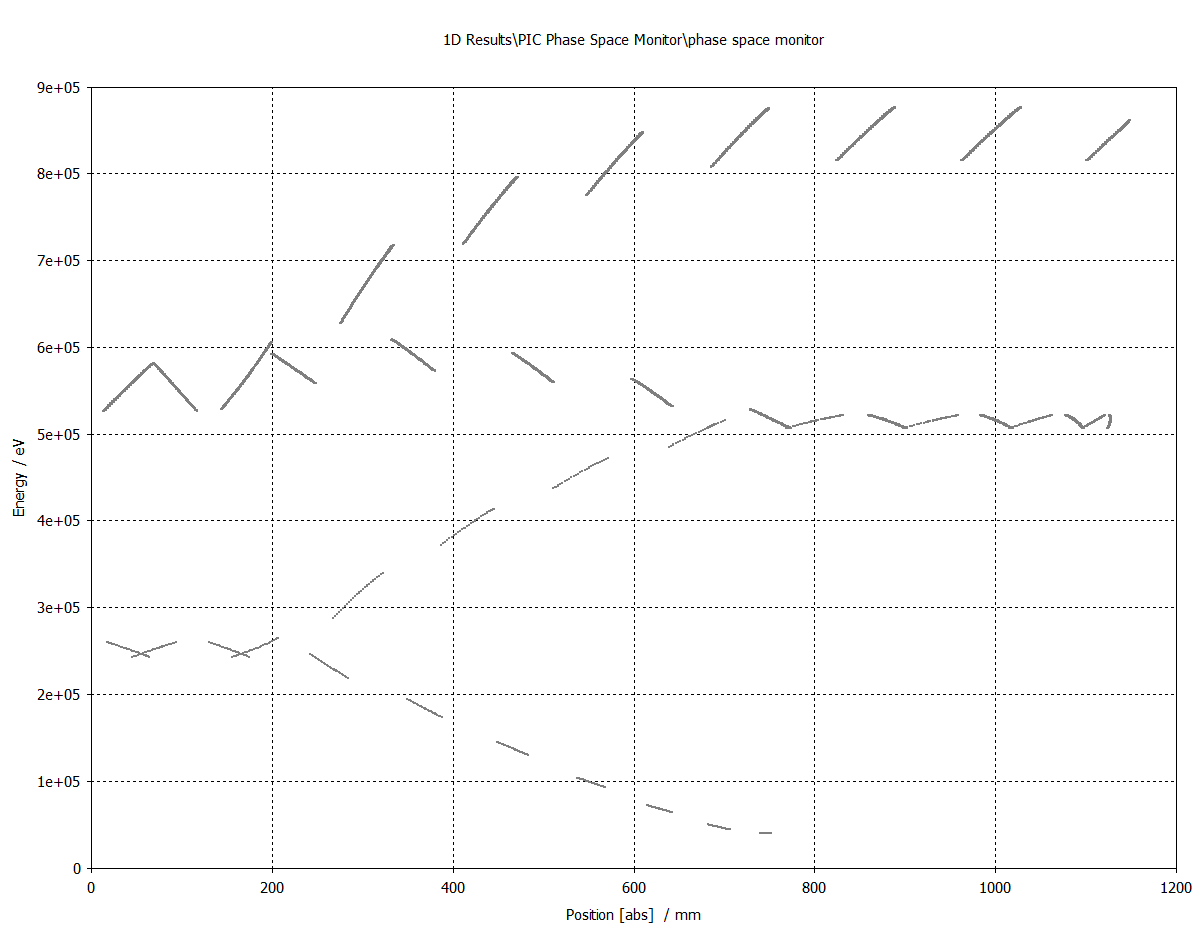
\includegraphics[width=\linewidth]{./figures/cst/cst_second_design3.png}
      \caption{Two pass simulation of \fromfig{initial_three_magnet_design}}
    \end{subfigure}
    \caption{$|r|$ vs $Energy$ simulation of initial design.}
    \label{fig:initial_designs_PIC_phase_space_monitor}
\end{figure}

The behavior of the beam in the \fromfig{initial_designs_PIC_phase_space_monitor} after the first pass indicates that phase stability is not maintained. 
When the simulation results are examined further, it was observed that the beam started the second pass at $t \approx 12$ ns after the injection. 
Considering the starting phase lag $\phi_{lag}=15^\circ$, this would mean phase lag of the second pass was $\phi_{lag2}=120^\circ$.
This result can be observed in \fromfig{initial_designs_PIC_phase_space_monitor}, as the beam decelerates after a short acceleration in the beginning of the second pass.

After various similar observations in \textit{CST} similations, underlying cause of this problem was thought to be the $L_{pass} = n \lambda$ approach on magnet design failing in low energies, 
as anticipated and discussed earlier in the \fromsec{parameter_sweep}.
\emph{The necessity for an alternative tool, capable of aiding researchers in improving beam behavior, was deemed evident.}

In KAHVELab, several improvements were made to these initial designs by \textit{Mr. Sinan ÖZ}. They include curved edges on cavity which reduce the power loss on cavity walls, and redesigned iron casing on magnets for ease of production and maintenance.
Improved designs can be seen in the figures below.
\begin{figure}[H]
    \captionsetup[subfigure]{justification=centering}
    \captionsetup{justification=centering}
    \centering
    \begin{subfigure}{.5\textwidth}
      \centering
      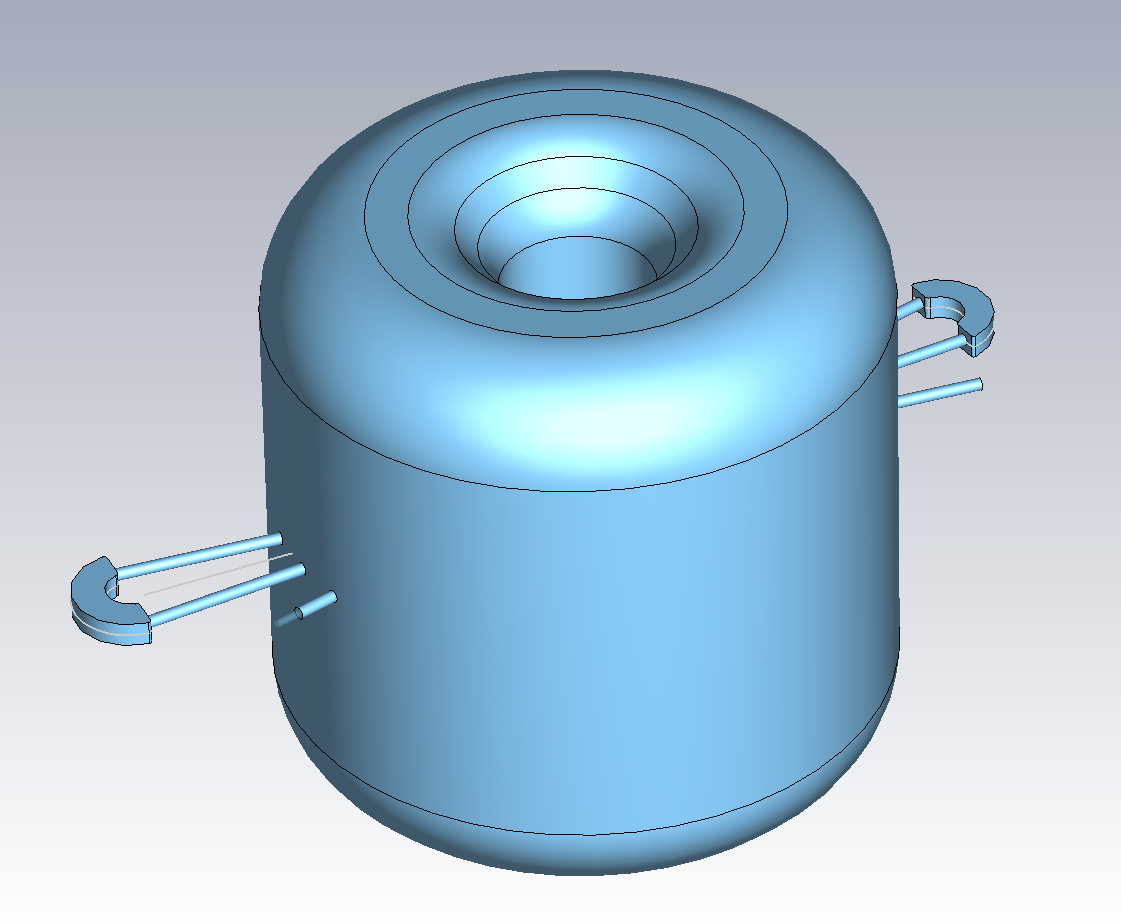
\includegraphics[width=.9\linewidth]{./figures/cst/cst_sinan_cavity_design1.png}
    \end{subfigure}%
    \centering
    \begin{subfigure}{.5\textwidth}
      \centering
      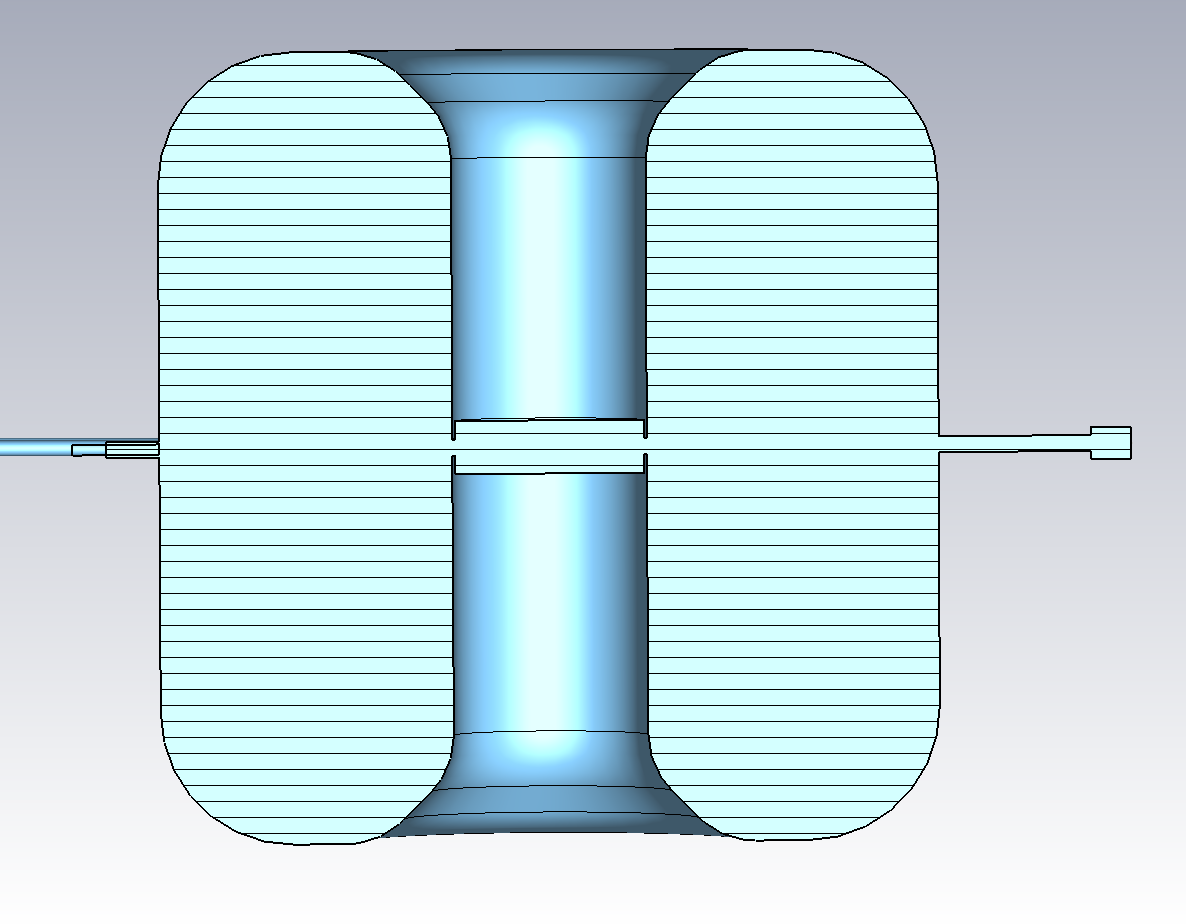
\includegraphics[width=.94\linewidth]{./figures/cst/cst_sinan_cavity_design2.png}
    \end{subfigure}
    \caption{Improved cavity design.}
    \label{fig:improved_cavity_design}
\end{figure}

\begin{figure}[H]
    \centering
    \captionsetup{justification=centering}
    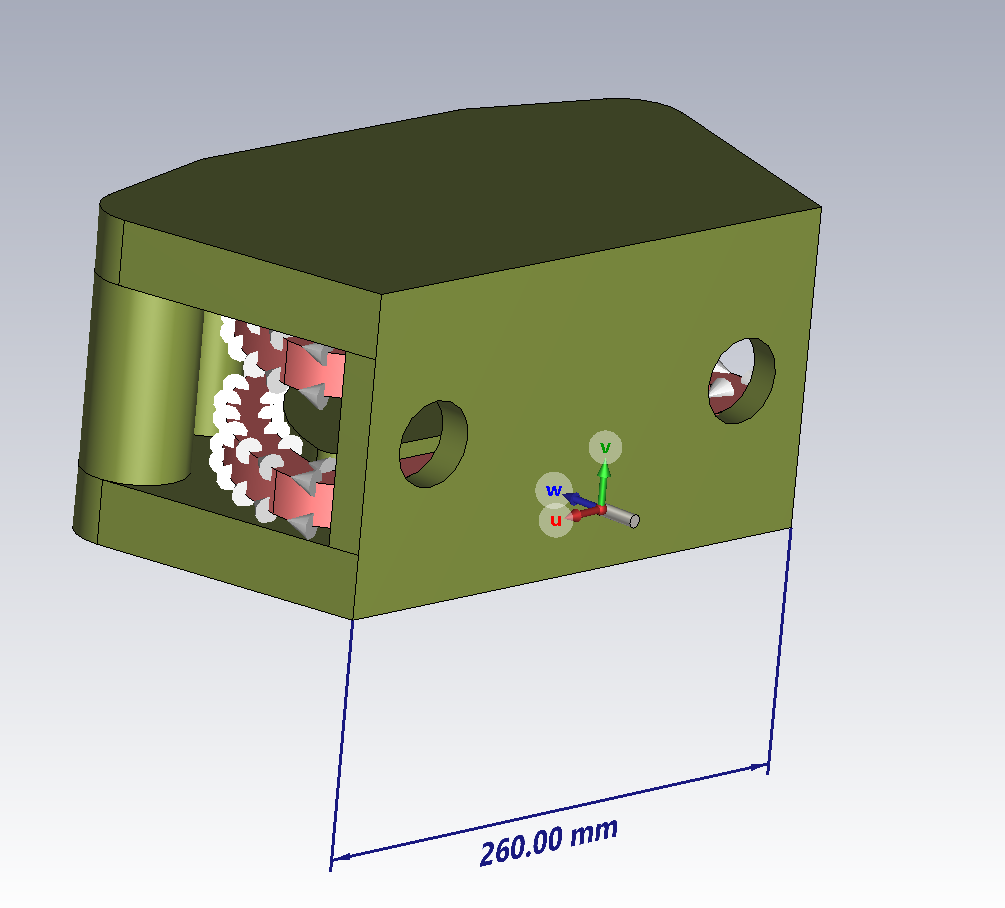
\includegraphics[width=.7\linewidth]{./figures/cst/cst_second_magnet_design1.png}
    \caption{Improved magnet design.}
    \label{fig:improved_magnet_design}
\end{figure}

\begin{figure}[H]
    \captionsetup[subfigure]{justification=centering}
    \captionsetup{justification=centering}
    \centering
    \begin{subfigure}{.5\textwidth}
      \centering
      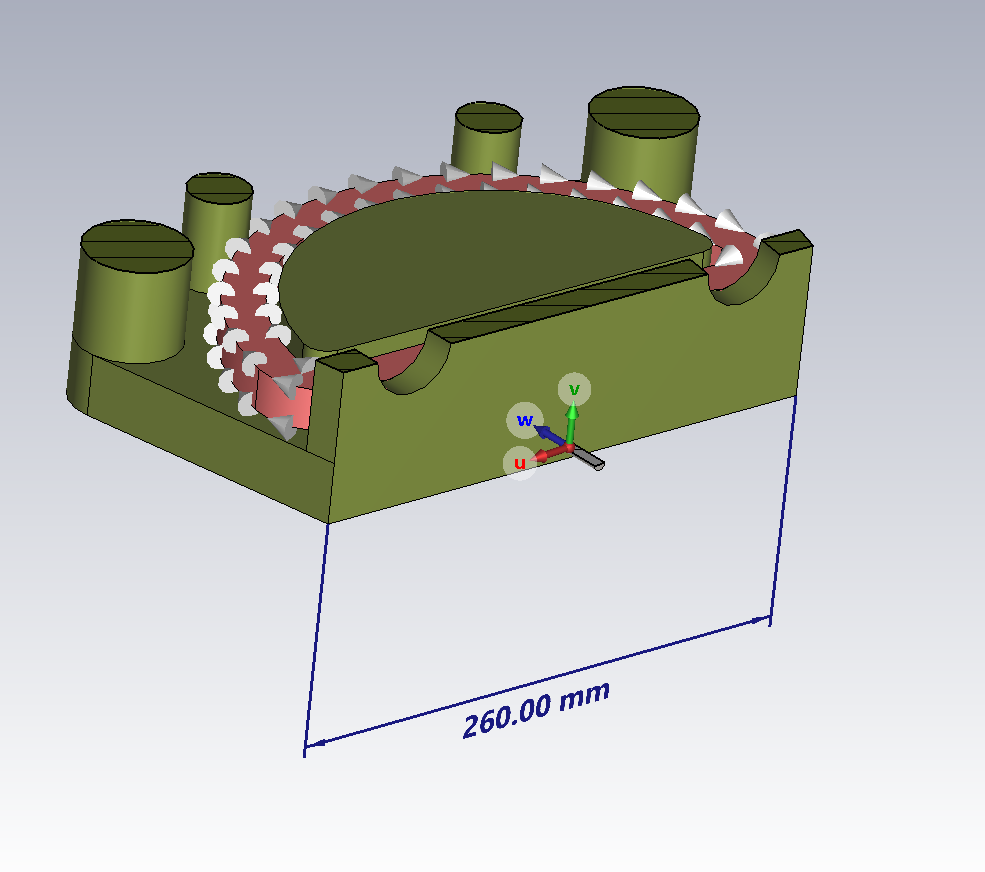
\includegraphics[width=.96\linewidth]{./figures/cst/cst_second_magnet_design2.png}
    \end{subfigure}%
    \centering
    \begin{subfigure}{.5\textwidth}
      \centering
      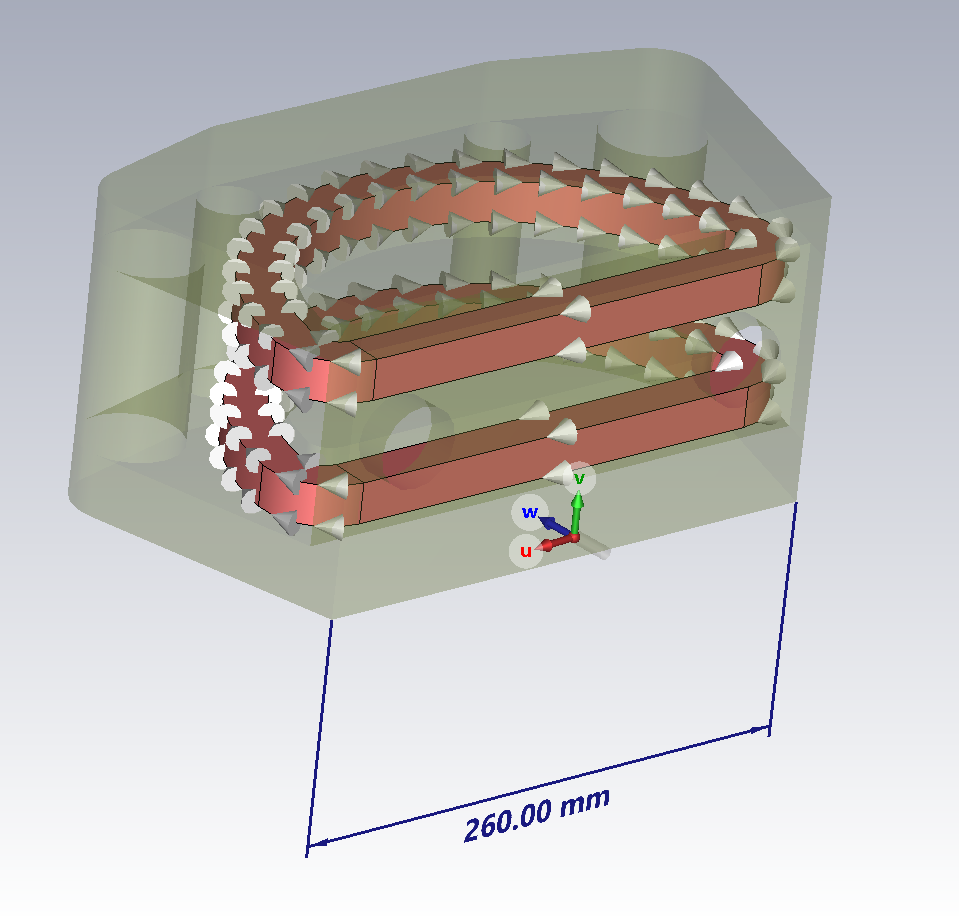
\includegraphics[width=.9\linewidth]{./figures/cst/cst_second_magnet_design3.png}
    \end{subfigure}
    \caption{Cross section and coils of improved magnet design.}
    \label{fig:improved_magnet_design_cross_section}
\end{figure}

\begin{figure}[H]
    \centering
    \captionsetup{justification=centering}
    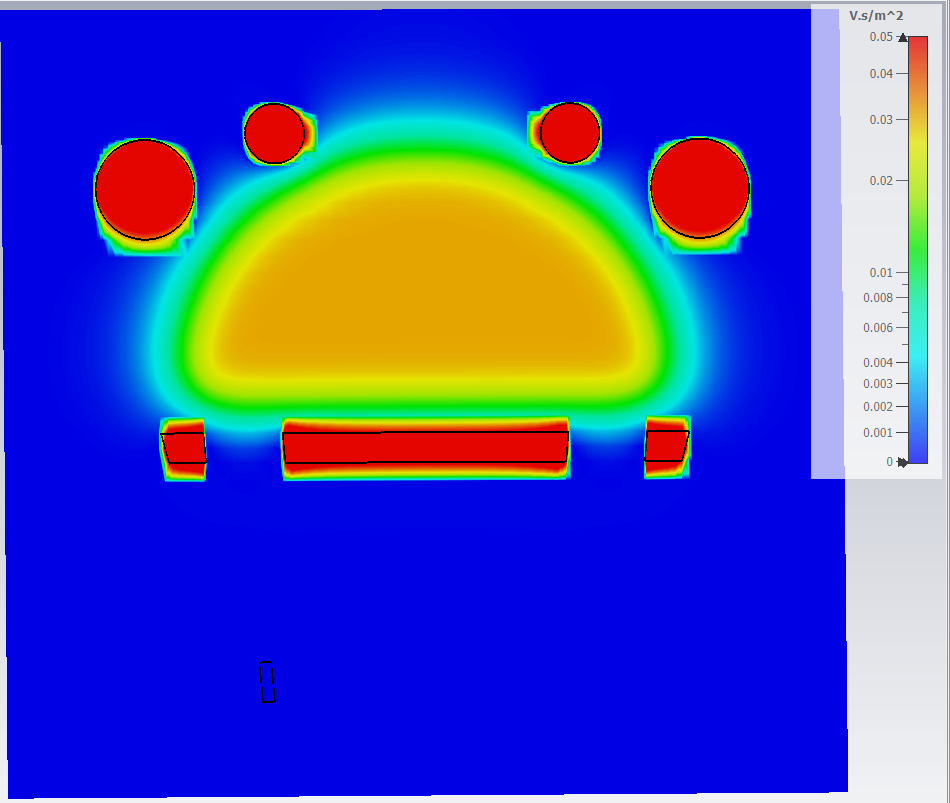
\includegraphics[width=.8\linewidth]{./figures/cst/cst_second_magnet_design4.png}
    \caption{Magnetic field in acceleration plate of improved magnet design.}
    \label{fig:improved_magnet_design_B}
\end{figure}


From \fromfigs{initial_magnet_design_B}{improved_magnet_design_B}, it can be observed that improved magnet design reduces magnetic field leak in enter and exit openings considerably. 
This reduction helps containing the spread of entering beam, decreasing the amount of focusing needed further into trajectory. 




\newpage

% START OF SIMULATION

\chapter{SIMULATION}
% Start of poc.tex
\section{Proof of Concept}
Once the need for a custom built tool for designing and simulating a Rhodotron type accelerator was apparent, a simple 1D proof of concept was implemented.

This proof of concept worked with interacting an electron with the EM field provided, at discrete time steps $dt$. The core sequence of this software is provided below.
Where $\vecthreeBF{r}$ is the position, $\vecthreeBF{v}$ is the velocity of the $e^-$;
\begin{itemize}
    \item Get electron energy $E_{in}$
    \item Get the RF field definitions
    \item Get the magnet design parameters if there is any
    \item Do following until the simulation time has ellapsed
    \begin{enumerate}
        \item Calculate $\vecthreeBF{E}_{||}$($\vecthreeBF{r}$)
        \item Calculate $\vecthreeBF{a}_{E ||}$ using \fromeq{para_and_perp_acc_of_lorentz_force}
        \item Calculate $\vecthreeBF{r}$($t+dt$) using \fromeq{leapfrog_sync_x}
        \item Calculate $\vecthreeBF{v}$($t+dt$) using \fromeq{leapfrog_sync_v}
        \item Calculate new $E_t$
    \end{enumerate}
\end{itemize}

The implemenation of this logic can be observed in the following code block.
\begin{figure}[H]
    \begin{minted}[linenos=true]{c++}
        for (double t=0; t<SimuTime; t+=dT){
            double RelBeta  = v/c;
            double RelGamma = 1.0 / sqrt(1.0-RelBeta*RelBeta);
        
            double ef=Eradial(r_pos*1000,t,0); // convert position to mm
            double acc=ef*1E6*eQMratio/(RelGamma*RelGamma*RelGamma); 
        
            r_pos = r_pos + v * dT*ns + 1/2*acc*(dT*ns)*(dT*ns);
            v = v + acc*dT*ns;

            RelBeta  = v/c;
            RelGamma = 1.0 / sqrt(1.0-RelBeta*RelBeta);
            Et=RelGamma*E0; 
        }
    \end{minted}
    \caption{Core logic loop of the POC}
    \label{fig:POC_core_logic}
\end{figure}

After simulating the \textit{synchronous electron} mentioned in \fromsec{cavity_of_a_rhodotron} with $\phi_{lag}=15^\circ$ for one pass in THE CAVITY, the results from \textit{POC}, \textit{CST} and \fromeq{W_gain_each_pass_pottier} are compared.
% 40 kW total power
% Emax = 0.96 in old, 2.08 in new version
% R1 = 0.1882
% R2 = 0.753
% f = 107.5
\begin{eqnarray}
    E_{Pottier} &=& 0.565 MeV \nonumber\\
    E_{CST} &=& 0.872 MeV \label{eq:poc_E_results}\\
    E_{POC} &=& 0.873 MeV \nonumber
\end{eqnarray}

As can be observed in \fromeq{poc_E_results}, \textit{POC software} and \textit{CST} produced very similar results. However, we cannot make the same claim regarding \fromeq{W_gain_each_pass_pottier}.
This inconsistency between $E_{Pottier}$ and $E_{CST}$ was noticed in the earlier simulations as well, which supported the idea of using another simulation software to reduce reliance on $CST$.
Using a single software would have made the process error prone. Their results, at the end of the day, depend heavily on the physical and mathematical models they use.

After the promising results obtained from \textit{POC}, the decision was made to develop a more robust simulation software. This software was named \textit{Rhodotron Simulation} for the current stage and started development in October, 2021.
The development and improvement efforts are still ongoing. 

During the development of \textit{Rhodotron Simulation} software, several intermediate builds have been implemented and tested. The following sections in this chapter investigates their implementations further.



\newpage


% Start of intermediate.tex
\section{Intermediate Versions}

\subsection{$L_{out}$ Optimization For Single $e^-$}
Initial step of improving $POC$ towards $Rhodotron Simulation$ was to implement \textit{$L_{out}$ optimizations} to help optimazing magnet designs, as discussed in \fromsec{parameter_sweep}.
First approach was to hang the $e^-$ outside of the cavity for $t_{out} = L_{out}/v$, then inject it back to the cavity with reversed $\vecthreeBF{v}$. Then sweep the $t_{out}$ parameter to find the optimal value.
This simple implementation can be found in \fromfig{lout_opt_single_e} of \fromapp{intermediate_codes}.

Although the results from this optimization sweep were promising after they were simulated with $CST$, simulating one particle would not be sufficiently useful for designing a magnet.

\subsection{$\phi_{lag}$ Optimization For Bunches}
After successfully accelerating single $e^-$, particle bunches were implemented to approximate a real $e^-$ gun. 
They were modeled as $N$ electrons fired from an $e^-$ gun at even time intervals. This approach was taken because the amount of time gun fires, defined as \textit{Gun Active Time, $t_g$}, is a crucial part of pulsing $e^-$ gun design.

Addition of bunches would immediately proven useful when finding optimal gun phase lag.
$\phi_{lag}$ for a bunch was defined as the RF phase when the first $e^-$ of the bunch entered the cavity, it defines the starting time of the current pass.
To use the \textit{parameter sweep} method, as used in \textit{$L_{out}$ optimization}, relevant bunch characteristics are defined as follows:

\begin{itemize}
    \item $\mu E$: Average energy
    \item $E_{RMS}$: Root mean square of energy
    \item $r_{RMS}$: Root mean square of $e^-$ positions
\end{itemize}

Optimal $\phi_{lag}$ would produce maximum $\mu E$ while minimizing $E_{RMS}$ \& $r_{RMS}$. For the first pass, 
$E_{RMS}$ and $r_{RMS}$ would be vaguely dependent of each other; therefore, early implementation of $\phi_{lag}$ sweep was based on minimizing $E_{RMS}$ during simulation (\textit{see \fromfig{phlag_opt}}). 
For $\mu E$ considerations, data from the software would be analyzed either manually or by using external tools such as $ROOT$. 

\begin{figure}[H]
    \centering
    \begin{minted}[linenos=true, autogobble, frame=lines, framesep=2mm, fontsize=\small]{c++}
        int phase_opt(int phase_sweep_range){
            double minrms = 1;
            int opt_phase;
            for(int RFphase = -phase_sweep_range; RFphase <= phase_sweep_range; RFphase++){
              Bunch bunch1(RFphase);
              double t1 = 0;
              bunch1.bunch_gecis_t(t1);
              bunch1.reset_pos();
        
              if( bunch1.E_rms() < minrms ){
                minrms = bunch1.E_rms();
                opt_phase = RFphase;
              }
            }
            return opt_phase;
        }
    \end{minted}
    \caption{$\phi_{lag}$ Optimization For Initial Bunch Design}
    \label{fig:phlag_opt}
\end{figure}

Since $\phi_{lag}$ is relatively easy to change after production, another version of \fromfig{phlag_opt} that was modified for given magnet design parameters was also implemented (\textit{see \fromfig{phlag_opt_n_pass} in \fromapp{intermediate_codes}}). 
This version can be useful for optimizing $\phi_{lag}$ in case of production issues in magnets. 

\subsection{$L_{out}$ Optimization For Bunches}




\newpage

% START OF APPENDIX

\appendix
\chapter{Intermediate Codes} \label{appendix:intermediate_codes}
\begin{figure}[H]
    \centering
    \begin{subfigure}{\textwidth}
        \centering
        \begin{minted}[linenos=true, autogobble, frame=lines, framesep=2mm]{c++}
            for(double i = 2; i < 9; i += dT_out){
                t_dum += i;
                double enow = gecis(r_pos, vel, Et, t_dum);
                if( enow > maxE ){
                  maxE = enow;
                  t_opt = i;
                }
                t_dum = t;
            }
        \end{minted}
    \end{subfigure} 
    \\
    \begin{subfigure}{\textwidth}
        \centering
        \begin{minted}[linenos=true, autogobble, frame=lines, framesep=2mm]{c++}
            double gecis(double r_pos, double vel, double Et, double &t){
                for(; r_pos >= -R2 && r_pos <= R2 ; t+=dT){
                    vel = c*sqrt(Et*Et-E0*E0)/Et;
                    double RelBeta  = vel/c;
                    double RelGamma = 1.0 / sqrt(1.0-RelBeta*RelBeta);
                
                    double ef=Eradial(r_pos*1000,t,RFphase*deg_to_rad);
                
                    double acc=ef*1E6*eQMratio/(RelGamma*RelGamma*RelGamma); 
                
                    r_pos = r_pos + vel * dT*ns + 1/2*acc*(dT*ns)*(dT*ns);
                    vel=vel+acc*dT*ns;
                    RelBeta  = vel/c;
                    RelGamma = 1.0 / sqrt(1.0-RelBeta*RelBeta);
                    Et=RelGamma*E0; 
                }
                return Et;
            }
        \end{minted}
    \end{subfigure}
    \caption{$L_{out}$ Optimization For Single $e^-$}
    \label{fig:lout_opt_single_e}
\end{figure}

\begin{figure}[H]
        \centering
        \begin{minted}[linenos=true, autogobble, frame=lines, framesep=2mm]{c++}
            int phase_opt(const vector<double>& Louts, int phase_sweep_range){
                double minrms = 1;
                int opt_phase;
                for(int RFphase = -phase_sweep_range; RFphase <= phase_sweep_range; RFphase++){
                    Bunch bunch1(RFphase);
                    double t1 = 0;
                    bunch1.bunch_gecis_t(t1);
                    bunch1.reset_pos();
            
                    for(int i = 0; i < Louts.size(); i++){
                        bunch1.bunch_gecis_d(Louts[i]);
                        bunch1.reset_pos();
                    }
                        
                    if( bunch1.E_rms() < minrms ){
                        minrms = bunch1.E_rms();
                        opt_phase = RFphase;
                    }
                }
                return opt_phase;
            }
        \end{minted}
    \caption{$\phi_{lag}$ Optimization For Tnitial Bunch Design}
    \label{fig:phlag_opt_n_pass}
\end{figure}


% END OF APPENDIX

% START OF BIBLIOGRAPHY

\begin{thebibliography}{9}

    \bibitem{rhodo_pottier}
    Jacques Pottier,
    \emph{A new type of rf electron accelerator: The rhodotron},
    Nuclear Instruments and Methods in Physics Research Section B: Beam Interactions with Materials and Atoms,
    Volumes 40–41, Part 2,
    1989,
    Pages 943-945,

    \bibitem{rhodo_prototype}
    J.M. Bassaler, J.M. Capdevila, O. Gal, F. Lainé, A. Nguyen, J.P. Nicolaï, K. Umiastowski,
    \emph{Rhodotron: an accelerator for industrial irradiation},
    Nuclear Instruments and Methods in Physics Research Section B: Beam Interactions with Materials and Atoms,
    Volume 68, Issues 1–4,
    1992,
    Pages 92-95,A:

    \bibitem{rhodos}
    Y. Jongen. (2001). \emph{Manufacturing of Electron Accelerators}. Ion Beam Applications s.a. (IBA) Chemin du Cyclotron 3, B-1348 Louvain-la-Neuve, Belgium.

    \bibitem{cpu_instruction_speed}
    Fukushima, Toshio. (2001). \emph{Reduction of Round-off Errors in Symplectic Integrators}. The Astronomical Journal. 121. 1768-1775. 

    \bibitem{cite:rhodo_design}
    W.~Kleeven, M.~Abs, J.~Brison, E.~Forton, J.~Hubert and J.~Van de Walle,
    \emph{Design and Simulation Tools for the High-Intensity Industrial Rhodotron Electron Accelerator},
    9th International Particle Accelerator Conference,
    2018
    
    
\end{thebibliography}

% END OF BIBLIOGRAPHY

\end{document}
